% !TEX program = xelatex
% !TEX options = --shell-escape -8bit -synctex=1
% !BIB program = biber
% !TEX encoding = UTF-8
% !TEX spellcheck = ru_RU

\documentclass[14pt, a4paper, oneside, russian]{extarticle}

\newif\ifDebug
%\Debugfalse
%\Debugtrue  % отображать отладочную информавцию на первых страницах


%   Настройка основного вида документа
%	Сделано на основании Положения о ВКР
%   Документ не редактировать!
%
%   Все изменеия вносить в custom_preampule.tex
%
%   Автор: Гаврилов А. Г.


%===================================================
% Настройка шрифтов и языка
%===================================================

\usepackage{fontspec}
\setmainfont{Times New Roman}
\setsansfont{Arial}
\setmonofont{Cascadia Code SemiLight}%[Scale=0.865] 
             

\usepackage{polyglossia}
\setdefaultlanguage[babelshorthands=true]{russian}
\setotherlanguage{english}


\setlength{\parindent}{1.25cm}

%===================================================
% Важные пакеты
%===================================================


\usepackage{etoolbox} %много вспомогательных команд
\usepackage{calc} % Добавляем пакет для команды \widthof еще он добавляет возможность вычисления длин типа 1in+6cm-10pt
\usepackage{totcount} %счетчики, сохраняющие значене между компиляциями
\usepackage{varwidth} %MinipageАвтоматическойШирины \begin{varwidth} \end{varwidth}
\usepackage{expl3}
\usepackage{amsmath, amssymb}

%===================================================
% Настройка полей
%===================================================
\usepackage{geometry}
\geometry{
	a4paper,
	left=30mm,
	right=15mm,
	top=20mm,
	bottom=20mm,
}

%===================================================
% Картинки
%===================================================

\usepackage{graphicx}
\graphicspath{{images}}
\usepackage{color}
\usepackage{tikz}

%===================================================
% Таблицы
%===================================================

\usepackage{longtable} %многостраничные таблицы
\usepackage{tabularx} %таблицы с полями автоширины 
\usepackage{array}


% Шрифт в таблицах (требования к оформлению ВКР 2026: 12 пт, одинарный интервал)
\AtBeginEnvironment{table}{%
	\def\insidetable{true}%
	\renewcommand{\arraystretch}{1.0}%
}
\AtEndEnvironment{table}{\renewcommand{\arraystretch}{1.5}}

\AtBeginEnvironment{tabular}{\ifdefined\insidetable\ifDebug\color{red}\fi\fontsize{12pt}{12pt}\selectfont\fi}
\AtBeginEnvironment{longtable}{\ifdefined\insidetable\ifDebug\color{red}\fi\fontsize{12pt}{12pt}\selectfont\fi}
\AtBeginEnvironment{tabularx}{\ifdefined\insidetable\ifDebug\color{red}\fi\fontsize{12pt}{12pt}\selectfont\fi}

\renewcommand{\arraystretch}{1.5} % межстрочный интервал вне таблиц float

%===================================================
% Математические формулы
%===================================================

\usepackage{amsmath}
\usepackage{amsfonts}

% Нумерация формул в пределах раздела: (2.1) справа (требования к оформлению ВКР 2026)
\numberwithin{equation}{section}
\renewcommand{\theequation}{\thesection.\arabic{equation}}
\makeatletter
\def\tagform@#1{\maketag@@@{(\ignorespaces#1\unskip)\hfil}}
\makeatother




%===================================================
% Verbatim
%===================================================

\usepackage{verbatim}
%===================================================
% Межстрочный интерва
%===================================================

\usepackage{setspace}
%\onehalfspacing % Межстрочный интервал 1.5
\setstretch{1.425}

%===================================================
% Отключение переносов слов
%===================================================

\usepackage[none]{hyphenat}


%===================================================
% Заголовки глав и параграфов
%===================================================

\setcounter{secnumdepth}{4} %Глубина вложенности заголовокв в документе
\setcounter{tocdepth}{3} % в оглавлении: section, subsection, subsubsection (без paragraph/subparagraph)

\usepackage{titlesec} % Для настройки заголовков
\titleclass{\paragraph}{straight}
\titleclass{\subparagraph}{straight}
\titleformat{\section}[block]
{\centering\bfseries} % Полужирный, по центру, прописные
{ГЛАВА \thesection.\ } % Нумерация с точкой
{0em} % Расстояние между номером и текстом
{\MakeUppercase} % Код перед заголовком
 % Расстояние после заголовка (2 интервала = 3ex при 1.5)

\titleformat{\subsection}[block]
{\centering\bfseries}
{\thesubsection.\ }
{0em}
{\MakeUppercase}

\titleformat{\subsubsection}[block]
{\centering\bfseries}
{\thesubsubsection.\ }
{0em}
{}

\titleformat{name=\section,numberless}[block]
{\centering\bfseries}
{}
{0em}
{\MakeUppercase}

\titlespacing*{name=\section,numberless}{0pt}{1.3em plus 3pt minus 2pt }{1.3em plus 3pt minus 2pt }


\titleformat{\paragraph}[block]
{\centering}
{\theparagraph. \ }
{0em}
{ }



\titlespacing*{\section}{0pt}{1.3em plus 3pt minus 2pt }{1.3em plus 3pt minus 2pt } % Отступы вокруг заголовка главы
\titlespacing*{\subsection}{0pt}{1.3em plus 3pt minus 2pt }{1.3em plus 3pt minus 2pt } % Отступы вокруг заголовка параграфа
\titlespacing*{\subsubsection}{0pt}{1.3ex plus 3pt minus 2pt }{1.3em plus 3pt minus 2pt } % Отступы вокруг заголовка параграфа
\titlespacing*{\paragraph}{0pt}{1em plus 3pt minus 2pt }{1em plus 3pt minus 2pt } % Отступы вокруг заголовка параграфа

%===================================================
% Стиль страниы и нумерация
%===================================================

\usepackage{fancyhdr}
\pagestyle{fancy}
\fancyfoot{} %пустой нижний колонтитул
\fancyhead{}%Отчищаем верхний колонтитул
\fancyhead[C]{\thepage} % Номер страницы по центру вверху
\renewcommand{\headrulewidth}{0pt} % Убираем черту


%\setlength{\headsep}{10pt}
%\setlength{\voffset}{1cm}
\setlength{\topmargin}{-1in + 13mm}
\setlength{\headheight}{4mm}
\setlength{\headsep}{3mm}
%наскоклько верний колонтиту выше страницы
%\setlength{\headheight}{\heightof{9}}
%\setlength


%переопределяем стиль plain который используется поумолчанию для страниц начала глав
\fancypagestyle{plain}{%
	\fancyfoot{} %пустой нижний колонтитул
	\fancyhead{}%Отчищаем верхний колонтитул
	\fancyhead[C]{\thepage} % Номер страницы по центру вверху
	\renewcommand{\headrulewidth}{0pt} % Убираем черту
%	\setlength{\headsep}{2ex}%наскоклько верний колонтиту выше страницы
%	\setlength{\headheight}{2ex}
}


%===================================================
% Подписи к рисункам, таблицам, листингу
%===================================================

%--- Настройка меток
\usepackage{caption}

%Разделитель номер рисунка
\DeclareCaptionLabelSeparator{dot}{.~}  
%Разделитель номер таблицы         
\DeclareCaptionLabelSeparator{dot_tbl}{.\\}            

%Подпись рис. центр
\captionsetup[figure]{
	name=Рис.,
	justification=centering,
	labelsep=dot, 
	format=plain,
	font={onehalfspacing},
	%skip=0ex, 
	belowskip=-2ex plus 4pt minus 2pt , 
	%aboveskip=1ex plus 4pt minus 2pt 
}                       

%Подпись табл. справа
\captionsetup[table]{
	name=Таблица,
	justification=raggedleft,
	labelsep=dot_tbl, 
	format=plain, 
	singlelinecheck=false,
	font={onehalfspacing},
	%belowskip=1ex plus 4pt minus 2pt, 
	%aboveskip=1ex  plus 4pt minus 2pt 
} 

%Подпись листинг. справа
\captionsetup[listing]{
	justification=raggedleft,
	labelsep=dot_tbl, 
	format=plain, 
	position=above, 
	singlelinecheck=false,
	font={onehalfspacing}, 
	%belowskip=1 ex plus 4pt minus 2pt , 
	aboveskip=-1.4ex  plus 4pt minus 2pt 
} 


%В рисунках и таблиц приложений используем префикс П
\appto\appendix{%
	\renewcommand{\thefigure}{\thesection.\arabic{figure}}
	\renewcommand{\thetable}{\thesection.\arabic{table}}
	\renewcommand{\thelisting}{\thesection.\arabic{listing}}
}


\renewcommand{\thefigure}{\thesection.\arabic{figure}}
\renewcommand{\thetable}{\thesection.\arabic{table}}


%привязываем счетки рисунков и таблиц к секциям (главам)
\usepackage{chngcntr}
\counterwithin{figure}{section}
\counterwithin{table}{section}

% Ссылки на рисунок и таблицу в тексте (требования к оформлению ВКР 2026)
\newcommand{\figref}[1]{Рис.~\ref{#1}}
\newcommand{\tabref}[1]{Таблица~\ref{#1}}


%===================================================
% Список литературы
%===================================================

\usepackage[style=gost-numeric, 
		sorting=none, 
		%defernumbers=true,
		]{biblatex}  
\addbibresource{vrkbibliograpgy.bib}
\urlstyle{same} 



\DeclareDelimFormat{multicitedelim}{\addcomma\space}
%\DeclareDelimFormat{compcitedelim}{\addcomma\space}

\defbibenvironment{bibliography}
{\list
	{\printfield{labelnumber}.\stepcounter{vkrTotalbooks}}
	{\toggletrue{bbx:gostbibliography}% %включаем ГОСТ 2018
		\renewcommand*{\revsdnamepunct}{\addcomma}%
		\renewcommand*{\labelnamepunct}{\addperiod\space}%
		\setlength{\labelwidth}{0pt}%
		\setlength{\leftmargin}{0em}%         % Красная строка для номера
		\setlength{\itemindent}{10.5mm}%        % Компенсируем отступ
		\setlength{\labelsep}{0.4em}%
		\setlength{\listparindent}{0pt}%
		\setlength{\itemsep}{\bibitemsep}%
		\setlength{\parsep}{\bibparsep}%
		\renewcommand*{\makelabel}[1]{\hss##1}}}
{\endlist}
{\item}

\renewcommand*{\mkgostheading}[1]{#1} %убираем курсив в спсике литературы


%===================================================
% Настройка оглавления
%===================================================


\usepackage{tocloft} % Для настройки оглавления

%Заголовок оглавления
\renewcommand{\cfttoctitlefont}{\hfill\bfseries}
\renewcommand{\cftaftertoctitle}{\hfill\vspace{1em}}

\renewcommand{\cftpnumalign}{r}


\cftsetrmarg{3ex}
\cftsetpnumwidth{3ex}

\renewcommand{\cftdotsep}{2}

\renewcommand{\cftsecpresnum}{ГЛАВА }
\setlength{\cftsecnumwidth}{\widthof{ГЛАВА 10.\ }}
\renewcommand{\cftsecaftersnum}{. }
\renewcommand{\cftsecleader}{\cftdotfill{\cftdotsep}}
\renewcommand{\cftsecfont}{\normalfont}        % обычный шрифт
\renewcommand{\cftsecpagefont}{\normalfont}    % шрифт номеров страниц
\setlength{\cftbeforesecskip}{0.0em} 


\setlength{\cftsubsecnumwidth}{\widthof{0.0.\ }}
\renewcommand{\cftsubsecaftersnum}{. } % Точка после номера параграфа
\renewcommand{\cftsubsecleader}{\cftdotfill{\cftdotsep}}
\renewcommand{\cftsubsecfont}{\normalfont}        % обычный шрифт
\renewcommand{\cftsubsecpagefont}{\normalfont}    % шрифт номеров страниц
\setlength{\cftbeforesubsecskip}{0.0em} 

\setlength{\cftsubsubsecnumwidth}{\widthof{0.0.0.\ }}
\renewcommand{\cftsubsubsecaftersnum}{. } % Точка после номера параграфа
\renewcommand{\cftsubsubsecleader}{\cftdotfill{\cftdotsep}}
\renewcommand{\cftsubsubsecfont}{\normalfont}        % обычный шрифт
\renewcommand{\cftsubsubsecpagefont}{\normalfont}    % шрифт номеров страниц
\setlength{\cftbeforesubsubsecskip}{0.0em} 

%Главы капсом
%https://tex.stackexchange.com/questions/156916/how-to-make-section-name-uppercase-in-toc
\makeatletter
%\patchcmd{\l@subsection}{#1}{\MakeUppercase{#1}}{}{}
%\patchcmd{\l@section}{#1}{\MakeUppercase{#1}}{}{}
\makeatother

% Уменьшить отступ перед номерами страниц

%===================================================
% Настройка приложений
%===================================================


% Переопределяем формат для приложений

\appto\appendix{%
	
	%\renewcommand{\thesection}{\arabic{section}} 
	
	\renewcommand{\thesection}{\Asbuk{section}} %почему то опять вернули буквы в приложения
	
	\titleformat{\section}[block]
	{\bfseries\raggedleft} % Полужирный, по центру, прописные
	{Приложение \thesection.} % Нумерация с точкой
	{0em} % Расстояние между номером и текстом
	{\\} % Код перед заголовком
	[\vspace{0ex}] 
	
	\titleformat{\subsection}[block]
	{\centering\bfseries}
	{\thesubsection.\ }
	{0em}
	{}
	
	{ }% Настройки оглавления для приложений
	\addtocontents{toc}{%
		\protect\renewcommand{\protect\cftsecpresnum}{Приложение }%
		\protect\setlength{\protect\cftsecnumwidth}{\widthof{Приложение М.\ }}%
		\protect\renewcommand{\protect\cftsecaftersnum}{.}%
	}
}

%Команды для разделов для прриложений
%Имеют номер, но не светятся в оглавлении
\newcommand{\hiddensubsection}[1]{%
	\addtocounter{subsection}{1}%
	\subsection*{\thesubsection. #1}%	
}

\newcommand{\hiddensubsubsection}[1]{%
	\addtocounter{subsubsection}{1}%
	\subsubsection*{\thesubsubsection. #1}%	
}



%===================================================
% Листинги кода
%===================================================


\usepackage[newfloat]{minted}
\setminted{linenos=false,
	style=vs,
	fontsize=\fontsize{14pt}{14pt},
	tabsize=3,
	frame=lines}
%\usepackage{listings}

%\ifn

\counterwithin{listing}{section}
\renewcommand{\thelisting}{\thesection.\arabic{listing}}
%\renewcommand{\listingscaption}{Листинг}  %для Minted без newfloat

%===================================================
% Настройка станартного положения рисунков
%===================================================

\usepackage{float}

% 1. Задаём [ht] для всех figure по умолчанию
\floatplacement{figure}{hbt} %в месте вызова или внизу станицы
\floatplacement{table}{hbt} %в месте вызова или внизу станицы
\floatplacement{listing}{hbt} %в месте вызова или внизу станицы

\setcounter{bottomnumber}{3}
\setcounter{topnumber}{2}

%счеткики для подсчета колчества рисунков и таблицу

\newcounter{vkrTotalfigures}
\newcounter{vkrTotaltables}

\AtBeginEnvironment{figure}{\stepcounter{vkrTotalfigures}}
\AtBeginEnvironment{table}{\stepcounter{vkrTotaltables}}

%расстояние между float (таблицы, рисунки) и текстом
\setlength{\floatsep}{1.6em plus 2pt minus 2pt}     % между float'ами
\setlength{\textfloatsep}{1.6em plus 2pt minus 2pt} % между float'ами и текстом
\setlength{\intextsep}{1.6em plus 2pt minus 2pt}    % для float'ов внутри текста


\SetupFloatingEnvironment{listing}{name=Листинг} 
%\renewcommand{\lstlistingname}{Листинг}

%для длинных листингов
\newenvironment{longlisting}{\vspace{\intextsep}\captionsetup{type=listing}}{}
\newenvironment{VKRlonglisting}{\vspace{\intextsep}\captionsetup{type=listing}}{}

%для длинных таблиц
\newenvironment{VKRlongtable}{\vspace{\intextsep-1ex}\stepcounter{vkrTotaltables}\begingroup\captionsetup{type=table}\def\insidetable{true}}{\endgroup}

\usepackage{placeins}  % Для команды \FloatBarrier

%===================================================
% Списки
%===================================================


\usepackage{enumitem} %упарвление списками

\setlist[enumerate]{nosep, leftmargin=1cm }  
\setlist[itemize]{nosep, leftmargin=1cm}

%\setlist[enumerate,1]{leftmargin=1.25cm +2ex + \labelsep }  
%\setlist[itemize,1]{leftmargin=1.25cm +2ex + \labelsep }

\setlist[enumerate,1]{leftmargin = \parindent }  
\setlist[itemize,1]{leftmargin = \parindent  }

% русские буквы в счетчике https://tex.stackexchange.com/questions/720496/how-to-make-cyrillic-alphabet-numbering-in-enumerate-with-enumitem-and-polygloss
\makeatletter
\AddEnumerateCounter{\asbuk}{\russian@asbuk@alph}{щ} % section 8.1
\makeatother



%===================================================
% Прочие плагины
%===================================================



\usepackage{lipsum}%для отладки текста, команда \lipsum
\usepackage{clipboard}
\usepackage{ifthen}

\usepackage{marginnote} %заметки на полях
\reversemarginpar 
\setlength{\marginparwidth}{25mm}
\usepackage[textsize=tiny]{todonotes}

\usepackage{refcount}  %всяукие команды для работы с ссылками, например \getpagerefnumber
\usepackage{metalogo}

%===================================================
% Отладка
%===================================================

\ifDebug
	\usepackage{layout} %Позволяет использовать команду \layout для печати структуры страницы
	\usepackage{layouts} %еще мног о команд для откладки
	\usepackage{showframe} %Рамки фокруг листа
	
	\AtBeginDocument{%
		\input{debug_page.tex}%
	}
	
\fi


%===================================================
% Добавляйте сюда ваши собственные пакеты и команды
%===================================================

% Ссылка на формулу в тексте (требования к оформлению ВКР 2026)
\newcommand{\formref}[1]{формула~\eqref{#1}}

% Блок расшифровки символов под формулой: все строки по левому краю
\newcommand{\formwhere}[1]{%
	\par\vspace{0.25\baselineskip}%
	\noindent
	#1%
	\par\vspace{0.25\baselineskip}%
}

\newcommand{\formwherenext}[2]{%
	\par\noindent #1~--- #2%
}



%===================================================
% Пакет hyperref. 
% Должен подключатся последним.
% Он необходим для работы с ссылками
% И меняет работу других пакетов
%===================================================


\usepackage{hyperref}
\hypersetup{hidelinks} %отключить посдветку ссылок
%\usepackage{bookmark} %для заклкдок



%===================================================
% Кастомные команды
%===================================================

%===========================
% Запись/чтение из aux

\makeatletter
% Команда для записи в .aux
\newcommand{\writetoaux}[2]{%
	
	\immediate\write\@auxout{%
		\string\global\string\@namedef{vkr#1}{#2}%
	}%
	
}
\makeatother

% Команда для чтения из .aux
\newcommand{\readfromaux}[1]{%
	\ifcsname vkr#1\endcsname
	\csname vkr#1\endcsname
	\else
	*Счетчик не определен или требуется перекомпиляция*%
	\fi
}

%===========================

%Красная маленькая заметка на полях

\newcommand{\vkrnote}[2][]{%
	\marginnote[{\fontsize{9pt}{9pt}\selectfont\fussy\color{red}#1}]%
	{{\fontsize{9pt}{9pt}\selectfont\setlength{\baselineskip}{9pt}\fussy\color{red}#2}}%
}


%===========================


%разбивка  строки на слова-строки
\ExplSyntaxOn
\NewDocumentCommand{\wordsperline}{m}
{
	\seq_set_split:Nnn \l_tmpa_seq { ~ } { #1 }
	\seq_use:Nn \l_tmpa_seq { \\ }
}
\ExplSyntaxOff

%Станкиновская шапка

\newcommand\vkrStandartHead%
{
	\begingroup
	\fontsize{12pt}{10pt}\selectfont
	{
		\centering
		\bfseries\noindent
		\includegraphics[width=54mm]{stankin-logo.pdf}\\
		МИНОБРНАУКИ РОССИИ\\
		федеральное государственное автономное образовательное учреждение\\
		высшего образования\\
		«Московский государственный технологический университет «СТАНКИН»\\
		(ФГАОУ ВО <<МГТУ <<СТАНКИН>>) \\
	}
	
	
	
	\vspace{-0.75em}\noindent\rule{\textwidth}{0.4pt}\vspace{2ex}
	
	\noindent	
%	\begin{minipage}[t]{0.3\textwidth}
%		\bfseries
%		Институт\\
%		Информационных\\
%		Технологий\\	
%	\end{minipage}
%	\hfill
%	\begin{minipage}[t]{\widthof{\bfseries Вычислительных систем}+1pt}
%		\bfseries
%		Кафедра\\
%		Информационных\\
%		Технологий и\\ 
%		Вычислительных систем\\	
%	\end{minipage}
	\begin{minipage}[t]{0.4\textwidth}
		\bfseries
		Институт\\\expandafter\wordsperline\expandafter{\vkrInstitute}
	\end{minipage}
	\hfill
	\begin{varwidth}[t]{0.3\linewidth}
		\bfseries\raggedright
		Кафедра\\
		\vkrKafedra
	\end{varwidth}
	\endgroup
}

\def\emptystr{}
%===========================
% Макросы для вставки должности регалий о руководителе или консультанте


%должность, степ. , зван.
\def\insertPersonInfo#1{%
	\edef\tmpZ{\csname vkr#1Position\endcsname}%
	\edef\tmpA{\csname vkr#1DegreeShort\endcsname}%
	\edef\tmpB{\csname vkr#1TitleShort\endcsname}%
	\tmpZ%
	\ifx\tmpA\empty\else%
	,\space\tmpA%
	\fi%
	\ifx\tmpB\empty\else%
	,\space\tmpB%
	\fi%	
}

%степ. , зван., если нет то должность
\def\insertPersonInfoA#1{%
	
	\edef\tmpZ{\csname vkr#1Position\endcsname}%
	\edef\tmpA{\csname vkr#1DegreeShort\endcsname}%
	\edef\tmpB{\csname vkr#1TitleShort\endcsname}%
	\ifx\tmpA\emptystr%
	\ifx\tmpB\empty%	
	\tmpZ%
	\else%
	Error In #1 info!%
	\fi%		
	\else%
	\tmpA%
	\ifx\tmpB\empty\else%
	,\space\tmpB%
	\fi%
	\fi%
}

%должность каф. , степ. , зван.
\def\insertPersonInfoB#1{%
	\edef\tmpZ{\csname vkr#1Position\endcsname}%
	\edef\tmpA{\csname vkr#1DegreeShort\endcsname}%
	\edef\tmpB{\csname vkr#1TitleShort\endcsname}%
	\tmpZ\space каф. \vkrKafedraShort%
	\ifx\tmpA\empty\else%
	,\space\tmpA%
	\fi%
	\ifx\tmpB\empty\else%
	,\space\tmpB%
	\fi%	
}


%===========================
%===========================
%===========================
%===========================
%===========================
%===========================
%===========================
%===========================
%===========================
%===========================
%===========================
%===========================
%===========================

%Включаем подссветку ссылок для откладки документа
\hypersetup{hidelinks=false}

%Настройка документа

%===================================================
% Информация о типе работы
%===================================================

\newif\ifVkrOfBachelor  %Флаг для определения типа работы
%\VkrOfBachelortrue     %работа бакалавра -  магистрам закоментировать!


%Тена вкр
\def\vkrTheme{Исследование методов автоматического составления расписания и разработка программного средства поддержки генерации расписания для МГТУ «СТАНКИН»}
%Направление
\def\vkrMajor{09.04.04} %09.03.01 09.03.04  09.04.01  09.04.04
\def\vkrMajorName{Программная инженерия}
%Профиль
\def\vkrSpesialization{Технологии разработки интеллектуальных систем и программных комплексов}
%

%Кафедра 
\def\vkrKafedra{информационных технологий и вычислительных систем}
\def\vkrKafedraShort{ИТиВС}

%Институт 
\def\vkrInstitute{информационных технологий}
\def\vkrInstituteShort{ИТ}

%Зав. кафедрой 
\def\vkrKafedraHead{Новоселова Ольга Вячеславовна}
\def\vkrKafedraHeadShort{Новоселова О.\,В.}
\def\vkrKafedraHeadTitles{к.т.н., доц.}

%===================================================
% Информация о студенте
%===================================================
\def\vkrStudentGroup{ИДМ-24-08}
\def\vkrStudent{Кочановский Кирилл Андреевич}
\def\vkrStudentR{Кочановского Кирилла Андреевича} %Родительный падеж
\def\vkrStudentShort{Кочановский К.\,А.}   % \, - короткий пробел 


%===================================================
% Информация о научном руководителе
%===================================================

\def\vkrAdvisor{Гаврилов Андрей Геннадьевич}
\def\vkrAdvisorShort{Гаврилов А.\,Г.}

%должность 
\def\vkrAdvisorPosition{доцент}  %ст. преподаватель, доцент, профессор или зав. кафедрой
\def\vkrAdvisorPositionShort{доц.}  %ст. преп., доц., проф., зав. каф.,

%ученое степень
\def\vkrAdvisorDegree{кандидат технических наук}  %кандидат или доктор  такиих то наук или пусто
\def\vkrAdvisorDegreeShort{к.т.н.}  %аббривииатура первых букв степени или пусто

%ученое звание 
\def\vkrAdvisorTitle{доцент}  %доцент, профессор (не путать с должностью!!, могут совпадать и отличаться) или пусто
\def\vkrAdvisorTitleShort{доц.}  %доц., проф. или пусто


%===================================================
% Информация о научном консультанте (для магистров)
%===================================================

\def\vkrConsultant{Тохунц Наталия Борисовна}
\def\vkrConsultantShort{Тохунц Н.\,Б.}

%должность 
\def\vkrConsultantPosition{доцент}  %ст. преподаватель, доцент, профессор или зав. кафедрой
\def\vkrConsultantPositionShort{доц.}  %ст. преп., доц., проф., зав. каф.,

%ученое степень
\def\vkrConsultantDegree{}  %кандидат или доктор  такиих то наук или пусто
\def\vkrConsultantDegreeShort{}  %аббривииатура первых букв степени или пусто
%ученое звание 
\def\vkrConsultantTitle{} %доцент, профессор (не путать с должностью!!, могут совпадать и отличаться) или пусто
\def\vkrConsultantTitleShort{}  %доц., проф. или пусто






\makeatletter
\setlength{\@fptop}{0pt}
\setlength{\@fpbot}{0pt plus 1fil}
\makeatother

\begin{document}

	\sloppy
	\hbadness=10000

	%Титульный лист
	\newpage
	\pagestyle{empty}
	\phantomsection
\pdfbookmark[1]{Титульный лист}{Титул}

\begingroup
\fontsize{12pt}{10pt}
\selectfont

\vkrStandartHead %%Шапка станкина

\vspace{2cm}


\begin{center}

	\bfseries
	{\fontsize{14pt}{12pt}\selectfont\vkrStudent}\\
	\hfill\\
	\normalfont
	Выпускная квалификационная работа\\
	по направлению подготовки \\
	\vkrMajor\space<<\vkrMajorName>>\\
	Профиль: <<\vkrSpesialization>> \vspace{1.5em}\hfill


	{

		\parbox{1\linewidth}{\centering\bfseries\fontsize{16pt}{16pt}\selectfont\MakeUppercase{\vkrTheme}}

		\vspace{1.5em}\hfill
		Регистрационный номер № \rule{3cm}{0.25pt}
	}
\end{center}



\vspace{1cm}

\noindent%
\begin{tabular}{
		@{}
		b{0.35\linewidth}
		@{}
		b{2.5cm}
		@{}
		b{2ex}
		@{}
		b{0.35\linewidth}
		}
	Зав. кафедрой  & \underline{\hspace{\linewidth}} & &	\vkrKafedraHeadTitles\strut\newline\vkrKafedraHeadShort \\
	Научный руководитель  &  \underline{\hspace{\linewidth}} & & 	\insertPersonInfoA{Advisor}\strut\newline\vkrAdvisorShort\strut \\
	\ifVkrOfBachelor
	\else
	Научный консультант &  \underline{\hspace{\linewidth}} & & \insertPersonInfoA{Consultant}\strut\newline\vkrConsultantShort\strut \\
	\fi
	Обучающийся &  \underline{\hspace{\linewidth}} & & \strut\newline\vkrStudentShort
\end{tabular}




\vfill


{\centering\bfseries Москва 2026\,г.\\}

\endgroup




	%Задание на ВКР
	\newpage
	\pagestyle{empty}
	\begingroup


\fontsize{12pt}{10pt}
\selectfont
\renewcommand{\arraystretch}{1}



\phantomsection
\pdfbookmark[1]{Задание на ВКР}{Задание на ВКР}

\vkrStandartHead

\vspace{1cm}

\hfill%
\begin{minipage}{0.5\linewidth}
	\raggedleft
	\textbf{<<УТВЕРЖДАЮ>>}\\
	Заведующий кафедрой ИТиВС\\
	\vkrKafedraHeadTitles\space\vkrKafedraHeadShort\\[3ex]
	\underline{\hspace{30mm}}\\
	<<\underline{\hspace{7mm}}>>\underline{\hspace{30mm}} 2026 г.
\end{minipage}

\vspace{0.5cm}

\begin{center}
	{\fontsize{14pt}{14pt}\selectfont\textbf{Задание}}

	на выполнение выпускной квалификационной работы \\
	по направлению подготовки \\
	09.04.04 <<Программная инженерия>>\\
	Профиль: <<Технологии разработки интеллектуальных систем и программных комплексов>>
\end{center}

{
	\centering\fontsize{14pt}{12pt}\selectfont
	\begin{tabular} {l l l}
		Студент группы \vkrStudentGroup    	& &  	Научный руководитель \\
		\vkrStudentShort					& & 	\insertPersonInfo{Advisor} \vkrAdvisorShort\\
	\end{tabular}\\
}

\begin{center}
	\bfseries\fontsize{14pt}{12pt}\selectfont
	\parbox{0.9\linewidth}{\centering Тема: <<\vkrTheme}

\end{center}

\vfill

\noindent Тема утверждена приказом <<\underline{\hspace{7mm}}>>.\underline{\hspace{30mm}} 202\_ г. № \_\_\_\_

\noindent Срок сдачи ВКР на кафедру <<\underline{\hspace{7mm}}>>.\underline{\hspace{30mm}} 202\_ г.

\newpage
\fontsize{12pt}{16pt}
\selectfont
\begin{enumerate} [nosep,font=\bfseries, left=0pt]
	\item \textbf{Описание задания на выполнение ВКР }
		\begin{enumerate} [nosep, label*=\arabic*.,font=\bfseries]
			\item \textbf{Тип ВКР --- исследовательская работа. }
			\item \textbf{Цель исследования --- повышение эффективности деятельности учебного заведения. }
			\item \textbf{Объект исследования --- программная поддержка процесса создания расписания учебных занятий. }
			\item \textbf{Предмет исследования --- архитектура и функционирование клиент-серверного веб-приложения для создания расписания учебных занятий с учётом личных предпочтений преподавательского состава. }
			\item \textbf{Методы исследования ---  системный анализ, процессно-ориентированный подход и функциональное моделирование процессов, объектно-ориентированный анализ. }
			\item \textbf{Задачи исследования:}
				\begin{enumerate} [nosep, label*=\arabic*.]
					\item Провести исследование различных методов автоматического составления расписаний учебных занятий. Сделать обоснованные выводы о наличии необходимости в разработке своего метода. Провести анализ правил составления расписания МГТУ «СТАНКИН».
					\item Обосновать требования для клиент-серверного веб-приложения для создания расписания учебных занятий.
					\item Разработать проект клиент-серверного веб-приложения для создания расписания учебных занятий.
					\item Разработать клиент-серверное веб-приложение для создания расписания учебных занятий в соответствии с разработанным проектом.
				\end{enumerate}
		\end{enumerate}
	\item \textbf{Требования к выполнению ВКР}
		\begin{enumerate} [nosep, label*=\arabic*.,font=\bfseries]

			\item \textbf{Соблюдение требований законодательной базы и стандартов}

				\begin{enumerate} [nosep, label*=\arabic*.]
					%===============================
					%  Выбрать  свою программу
					%===============================

					\item Образовательная программа высшего образования в магистратуре ФГБОУ ВО «МГТУ «СТАНКИН» по направлению подготовки 09.04.04 «Программная инженерия» для направленности (профиля) подготовки «Технологии разработки интеллектуальных систем и программных комплексов» (утв. 31.05.2021).

					\if 0  %это такой хитрый способ сделать многострочный коментарий

					\item  Образовательная программа высшего образования по направлению подготовки 09.03.01 Информатика и вычислительная техника : направленность (профиль) «Разработка программных комплексов в рамках цифровой трансформации деятельности предприятий» : уровень высшего образования бакалавриат : форма обучения очная  / ФГБОУ ВО «МГТУ «СТАНКИН». --- Москва, 2022 --- одобрена Учёным советом Университета 23.04.2022, утв. ректором Серебренным В.В 29.04.2022  --- (изменена и дополнена).

					\item Образовательная программа высшего образования по направлению подготовки 09.03.04 Программная инженерия : направленность (профиль) «Системный анализ и проектирование программных комплексов» : уровень высшего образования бакалавриат : форма обучения очная / ФГБОУ ВО «МГТУ «СТАНКИН». --- Москва, 2022 --- одобрена Учёным советом Университета 23.04.2022, утв. ректором Серебренным В.В 29.04.2022  --- (изменена и дополнена).

					\item Образовательная программа высшего образования по направлению подготовки 09.04.01 Информатика и вычислительная техника : направленность (профиль) «Управление программными продуктами и проектами» : уровень высшего образования магистратура : форма обучения очная / ФГБОУ ВО «МГТУ «СТАНКИН». --- Москва, 2022 --- одобрена Учёным советом Университета 23.04.2022, утв. ректором Серебренным В.В 29.04.2022  --- (изменена и дополнена).

					\item Образовательная программа высшего образования по направлению подготовки 09.04.03  Программная инженерия : направленность (профиль) «Технологии разработки интеллектуальных систем и программных комплексов» : уровень высшего образования магистратура : форма обучения очная / ФГБОУ ВО «МГТУ «СТАНКИН». --- Москва, 2022 --- одобрена Учёным советом Университета 23.04.2022, утв. ректором Серебренным В.В 29.04.2022  --- (изменена и дополнена).

					\fi

					%===============================
					%  Общая часть
					%===============================

					\item   П 01-04/7/2024. Положение о государственной итоговой аттестации по образовательным программам высшего образования --- программам бакалавриата, программам специалитета и программам магистратуры  --- утверждено приказом ректора от 03.04.2024\,г. №700/1. ---  ФГБОУ ВО «МГТУ «СТАНКИН».

					\item П 01-04/9/2024. Положение о выпускной квалификационной работе обучающихся по образовательным программам высшего образования --- программам бакалавриата, программам специалитета, программам магистратуры   --- утверждено приказом ректора от 02.09.2024. №700/1. --- ФГБОУ ВО «МГТУ «СТАНКИН».

				\end{enumerate}

			\item \textbf{Дополнительные требования}

				\begin{enumerate} [nosep, label*=\arabic*.]
					\item 	Оформление раздела «Список литературы» по национальному стандарту ГОСТ Р 7.0.100-2018 <<Библиографическая запись. Библиографическое описание. Общие требования и правила составления>>
					\item Результаты исследования должны быть опубликованы в виде научных статей и тезисов докладов (не менее 2), а также доложены на научно-технических конференциях и семинарах.
				\end{enumerate}
		\end{enumerate}

	\item \textbf{Срок сдачи оформленной квалификационной работы на кафедру --- вторая декада мая 2026\,г. }

\end{enumerate}

\vspace{3ex}%


\noindent%
\begin{tabularx}{\linewidth}{ @{} X @{}  l  @{}    }

	Исполнитель 							&  \vkrStudentShort   \\[3ex]

	Научный руководитель             		& 					   \\
    \insertPersonInfoB{Advisor} 	 		&   \vkrAdvisorShort
\end{tabularx}


\endgroup




	%Аннотация
	\newpage
	\pagestyle{empty}
	\phantomsection
\pdfbookmark[1]{Аннотация}{Аннотация}

\begin{center}
	\section*{Аннотация}

	выпускной квалификационной работы \\
	студента группы \vkrStudentGroup\space ФГАОУ ВО «МГТУ «СТАНКИН» \\
	\textbf{\vkrStudentR} \\
	по направлению подготовки \\
	\textbf{\vkrMajor «\vkrMajorName»} \\
	на тему: \\
	\textbf{«\vkrTheme»}

\end{center}

\subparagraph{Актуальность работы.} Формирование расписания учебных занятий является одной из основных и наиболее сложных задач автоматизации управления учебным процессом любого учебного заведения. МГТУ «СТАНКИН» не является исключением, каждый семестр специальный отдел в составе Учебно-методического управления МГТУ «СТАНКИН» \cite{stankin:schedule} составляет расписание на следующие полгода, выкладывает его на сайт университета и отправляет преподавателям и старостам групп. На сегодняшний день процесс создания расписания учебных занятий производится вручную, что является медленным и ресурсозатратным процессом. В данной выпускной квалификационной работе будет проведён анализ существующих подходов к решению данной задачи, а также предложен новый алгоритм решения. Финальным шагом работы будет разработка клиент-серверного веб-приложения для создания расписания университета.

\subparagraph{Научная новизна} работы состоит в разработке собственного алгоритма решения задачи составления расписания для учебного заведения ранее не исследованном методом, с возможностью тонкой настройки таких параметров, как процент окон, распределение количества учебных занятий по дням недели и в течение дня и многие другие менее значительные оптимизации.

\subparagraph{Практическая ценность} работы состоит в автоматизации такого ресурсозатратного процесса как планирование и формирование плана учебных занятий на семестр.

\edef\apppages{\fpeval{\getpagerefnumber{vkr:End} - \getpagerefnumber{vkr:AppendixBegin} + 1}}
\edef\totalpages{\getpagerefnumber{vkr:End}}
\edef\figures{\readfromaux{vkrTotalfigures}}
\edef\tables{\readfromaux{vkrTotaltables}}
\edef\books{\readfromaux{vkrTotalbooks}}

\subparagraph{Структура работы.} Выпускная квалификационная работа (ВКР) содержит \totalpages{}  стр.  сквозной нумерации. Количество рисунков в работе --- \figures, таблиц --- \tables. Позиций в списке литературы --- \books.

\subparagraph{Выводы:}

\begin{enumerate}
	\item Проведён анализ методов автоматического составления расписания и обоснован выбор гибридного подхода --- WFC для первичного допустимого решения и эволюционная оптимизация на основе генетического алгоритма для его улучшения.
	\item Разработаны требования к расписанию, описан предложенный алгоритм генерации и оптимизации, спроектирована архитектура и стек технологий клиент-серверного приложения и реализовано программное средство с веб-интерфейсом.
	\item Выполнено экономическое обоснование целесообразности внедрения разработанного средства для МГТУ «СТАНКИН».
\end{enumerate}

\subparagraph{Список работ, опубликованных по теме ВКР:}

\begin{enumerate}
	\item Работа, опубликованная на студенческой научно-практической конференции «Автоматизация и информационные технологии (АИТ-2024)» МГТУ «СТАНКИН» --- «Исследование методов автоматического составления расписания» \cite{ait2024}.
	\item Работа, опубликованная на 68-й Всероссийской научной конференции МФТИ --- «Алгоритм решения задач составления расписания занятий в образовательных учреждениях» \cite{mipt68conf}.
\end{enumerate}


	%Оглавление
	\newpage
	\pagestyle{fancy}
	\input{toc.tex}

	%Перечень сокращений и специальных терминов
	\newpage
	\pagestyle{fancy}
	\phantomsection
\section*{Перечень сокращений и специальных терминов}
\addcontentsline{toc}{section}{Перечень сокращений и специальных терминов}

\textbf{Сокращения}

\begin{description}
	\item[UI] User Interface – пользовательский интерфейс
	\item[WASM] WebAssembly — бинарный формат, запускаемый в браузере
	\item[БВО] Базовое высшее образование – соответствует бакалавриату и специалитету
	\item[СВО] Специализированное высшее образование – уровень, на котором реализуются программы магистратуры, ординатуры и ассистентуры-стажировки
	\item[СУБД] система управления базами данных
\end{description}

\textbf{Термины}

\begin{description}
	\item[Fitness function] функция приспособленности — критерий качества решения в оптимизации или ML
	\item[Бекэнд] часть программного обеспечения или веб-приложения, отвечающая за серверную логику, обработку данных и взаимодействие с базами данных
	\item[Фреймворк] структурированный набор инструментов и библиотек, облегчающий разработку программного обеспечения
	\item[Хостинг] услуга или платформа для размещения веб-сайтов и приложений на сервере, обеспечивающая их доступность в сети Интернет
\end{description}


    %Введение
	\newpage
	\pagestyle{fancy}
	\phantomsection
\addcontentsline{toc}{section}{ВВЕДЕНИЕ}

\section*{Введение}

Формирование расписания учебных занятий является одной из основных и наиболее сложных задач автоматизации управления учебным процессом вуза. Каждый семестр специальный отдел в составе Учебно-методического управления МГТУ «СТАНКИН» \cite{stankin:schedule} составляет расписание на следующие полгода, выкладывает его на сайт университета и отправляет преподавателям и старостам групп. На сегодняшний день процесс создания расписания учебных занятий производится вручную, что является медленным и ресурсозатратным действием.

\textbf{Целью} выпускной квалификационной работы является повышение эффективности деятельности учебного заведения за счёт исследования методов автоматической генерации расписания и разработки программного средства, реализующего такую генерацию с учётом регламента вуза, предпочтений преподавателей и «компоновки вуза».

\textbf{Объектом} исследования является программная поддержка процесса создания расписания учебных занятий.

\textbf{Предметом} исследования являются архитектура и функционирование клиент-серверного веб-приложения для создания расписания учебных занятий с учётом личных предпочтений преподавательского состава.

Для достижения цели поставлены следующие \textbf{задачи}:
\begin{enumerate}
	\item провести исследование методов автоматического составления расписаний учебных занятий, обосновать необходимость собственного подхода и проанализировать правила составления расписания МГТУ «СТАНКИН»;
	\item сформулировать требования к клиент-серверному веб-приложению для создания расписания учебных занятий;
	\item разработать проект клиент-серверного веб-приложения;
	\item реализовать клиент-серверное веб-приложение в соответствии с разработанным проектом.
\end{enumerate}

\textbf{Методы исследования:} системный анализ, процессно-ориентированный подход и функциональное моделирование процессов, объектно-ориентированный анализ, сравнительный анализ алгоритмов и программная реализация предложенного решения.

В работе будут рассмотрены методы автоматического создания расписания, предложен гибридный алгоритм на основе коллапса волновой функции (WFC) и эволюционной оптимизации, а также реализован сервис, выполняющий следующие функции:
\begin{enumerate}
	\item генерация расписания с учётом учебных планов, нормативов, списков преподавателей, групп и т.~д.;
	\item настройка распределения занятий по неделе и в течение дня, в том числе формирование разгрузочных дней и смещение учебного процесса в пределах суток;
	\item «компоновка вуза» для сокращения времени на переходы между учебными занятиями;
	\item вывод расписания в различных форматах, включая веб-интерфейс для просмотра преподавателями и студентами.
\end{enumerate}

Так как качество расписания определяет эффективность учебного процесса, значительное внимание уделено оценке расписаний и их последующему улучшению.

\textbf{Научная новизна} заключается в адаптации WFC к модели «группа~$\times$~день~$\times$~слот» с учётом регламента вуза и в гибридной схеме оптимизации: построение допустимого по жёстким ограничениям расписания с последующим улучшением эволюционным методом с repair-мутациями и отдельным этапом назначения аудиторий.

\textbf{Практическая ценность} состоит в автоматизации ресурсозатратного процесса планирования учебных занятий на семестр и в снижении числа нарушений нормативов при пересборке расписания.

\textbf{Структура работы.} Первая глава содержит обзор методов решения задачи. Во второй главе сформулированы требования к расписанию и описан предложенный алгоритм. Третья и четвёртая главы посвящены архитектуре и выбору средств реализации. Пятая глава описывает программную реализацию и результаты экспериментов. Экономическое обоснование приведено в отдельной главе. В заключении подведены итоги и намечены направления дальнейшей работы.


	%Глава1
	\newpage
	\pagestyle{fancy}
	\section{Анализ предметной области}


\subsection{Анализ методов автоматического создания расписания учебных занятий}

Задача создания расписания сводится к формированию и оптимизации процесса обслуживания конечного множества требований (заявок) на осуществление действий в системе. Задача составления расписания учебного заведения относится к классу NP-hard задач, она сводится к распределению трёх ресурсов: преподавательского состава, студенческого состава и аудиторий учебного заведения. Детальная постановка задачи, требования к расписанию и предлагаемый алгоритм приводятся во второй главе? в настоящей главе рассматриваются существующие методы решения и обосновывается выбор гибридного подхода.

Если посмотреть на количество научных статей (см. \figref{fig:relevance}), публикуемых международным сообществом на эту тему за последние пару десятков лет \cite{vrielink:patat2016}, то можно сделать вывод, что область образовательной логистики всё ещё является актуальной темой исследований и разработки.

\begin{figure}[H]
	\centering
	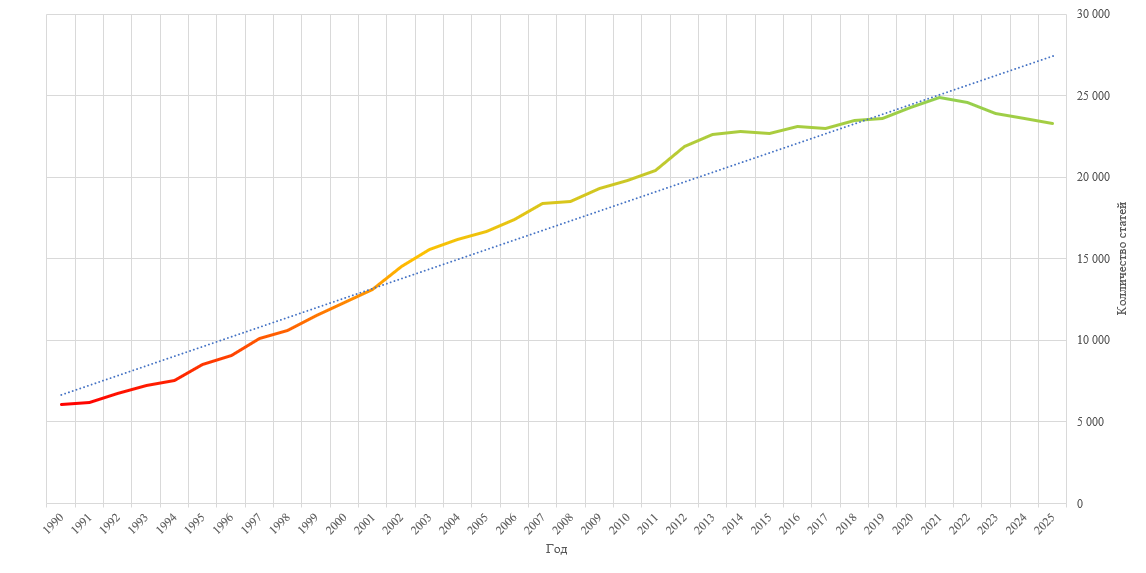
\includegraphics[width=1\textwidth]{images/ch1/relevance.png}
	\caption{Количество статей по годам на тему расписаний в высших учебных заведениях в Google Scholar по поисковому запросу «(timetabling OR timetable) AND higher education»}
	\label{fig:relevance}
\end{figure}

Для того, чтобы разобраться на каком этапе сейчас эта область, стоит проанализировать различные подходы и выявить основные тенденции и идеи.

\subsubsection{Линейные и целочисленные программные методы составления расписания}

Одними из первых, кто предоставил стратегии раскраски графов для решения проблемы составления расписания были Уэлш и Пауэлл (1967) \cite{welsh:chromatic}. Они заложили основу для более сложных исследований графовых эвристик в составлении расписания \cite{merlot:hybrid}. Эвристики составления расписания на основе раскраски графов - это полезный метод, на котором строится их оценка и улучшение.

Линейные и целочисленные программные методы - это математические алгоритмы, которые присваивают целочисленные значения переменным. Вариации этого метода были и до сих пор широко используются для решения комбинаторных задач оптимизации. Эти методы включают в себя программирование с ограничениями и методы удовлетворения ограничений.

Однако такие методы, как правило, требуют больших вычислительных ресурсов из-за экспоненциального количества переменных.

\subsubsection{Метаэвристики}

Метаэвристика --- это метод оптимизации, многократно использующий простые правила или эвристики для достижения оптимального или субоптимального решения. С 1995 по 2010 годы методологические подходы к решению проблем составления расписания обычно классифицировались на две категории метаэвристик: популяционные и одиночные \cite{burke:timepredefined}. Если классифицировать основные подходы и алгоритмы, то можно построить следующий график (см. \figref{fig:metaheuristics}).

\begin{figure}[H]
	\centering
	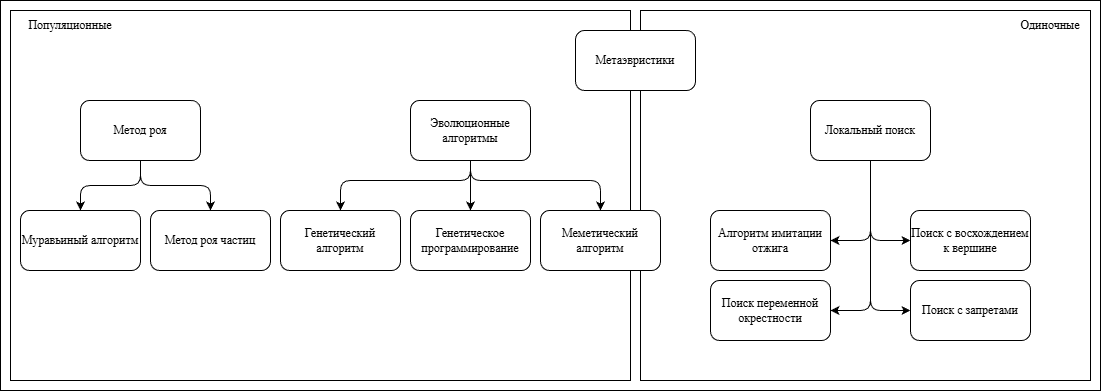
\includegraphics[width=1\textwidth]{images/ch1/metaheuristics.png}
	\caption{Классификация алгоритмов решения задачи}
	\label{fig:metaheuristics}
\end{figure}

Метаэвристический подход позволяет быстро получить приемлемое решение популяционным алгоритмом, а впоследствии улучшать его и удовлетворять дополнительные ограничения итеративным образом с помощью одиночных методов локального поиска.

Естественно нет возможности окунуться с деталями в каждый подход, но стоит хотя бы поверхностно изучить и оценить разные метаэвристические методы.

\paragraph{Локальные алгоритмы}

\subparagraph{Поиск с запретами.}

Поиск с запретами (Tabu search) относится к методологиям локального поиска и основан на поиске градиентного спуска. Существует несколько актуальных работ, в которых проведено ценное исследование методов поиска с запретами \cite{digaspero:tabu,petrovic:trajectories}. Исследования основаны на диверсификации соседей, при котором поиск расширяется для нахождения большего количества локальных оптимумов. Это приводит к интенсификации шагов и более быстрого нахождения решения.

Однако поиск с запретами имеет тенденцию застрять в подоптимальных областях или плато. Подоптимальные области - это регионы пространства поиска, где текущее решение локально оптимально, но не обязательно глобально. Плато представляют собой плоские области функции, где градиент близок к нулю, что затрудняет продвижение поиска.

\subparagraph{Алгоритм имитации отжига.}

Алгоритм SA --- это ещё один метод локального поиска. SA вдохновлён физическим процессом отжига металла, при котором нагреваемый металл постепенно остывает, обеспечивая более устойчивую кристаллическую структуру. В контексте оптимизации, этот метод направлен на поиск более широкой области пространства поиска, в которой принимаются худшие шаги и допускается более широкий поиск оптимального решения. Существует множество вариаций SA \cite{burke:timepredefined,dowsland:simulatedannealing}, он часто комбинируется с алгоритмом восхождения к вершине \cite{qu:survey}, или программированием с ограничениями \cite{brailsford:csp}.

Идеи стохастического локального поиска, заложенные в SA, используются в предлагаемом алгоритме на этапе оптимизации расписания при реализации repair-мутаций и локального поиска по целевой функции.

\paragraph{Эволюционные алгоритмы}

\subparagraph{Генетические алгоритмы.}

Среди эволюционных алгоритмов одними из самых изученных и популярных являются генетические алгоритмы (Genetic algorithms) \cite{corne:evolutionary}. Эти алгоритмы моделируют процесс естественного отбора, таким образом находя более совершенную форму «жизни».

\subparagraph{Меметические алгоритмы.}

Как дополнение к генетическим алгоритмам рассматриваются меметические алгоритмы \cite{burke:memetic}. Меметические алгоритмы (Memetic algorithms) представляют собой эволюционный метод оптимизации, который объединяет генетические алгоритмы с понятием «мема» из теории эволюции Ричарда Докинза. В данном контексте мем --- это небольшая единица знания или идеи, которая может передаваться от одного индивида к другому.

\subparagraph{Муравьиный алгоритм.}

Другой метод, основанный на популяции и более подробно исследованный в последнее десятилетие --- это группа муравьиных алгоритмов (Ant algorithms) \cite{dorigo:aco}. Эти алгоритмы отслеживают информацию, собранную в процессе поиска, и затем используют эту информацию для создания новых решений на следующих этапах.

\subsubsection{Гиперэвристики}

Как для подходов, основанных на одиночных решениях, так и для подходов, основанных на популяции, характерны свои недостатки. В последнее время большинство исследователей в области составления расписаний сосредотачивались на локальных или одиночных решениях, а не на алгоритмах, основанных на популяции \cite{albetar:harmony}.

Развитием, вытекающим из стандартных локальных и населённых решений проблем составления расписаний, является применение гиперэвристик. Гиперэвристики представляют собой метод поиска, в котором несколько эвристик объединяются и адаптируются. Различие между метаэвристиками и гиперэвристиками заключается в том, что гиперэвристики стремятся найти общепринятую методологию, а не решать конкретный экземпляр проблемы.

\subsection{Выводы по первой главе}

Был проведён анализ подходов к автоматическому составлению расписаний в высших учебных заведениях по обзорной литературе. Задача относится к классу NP-hard; точные методы (целочисленное программирование, SAT/SMT) применимы для проверки выполнимости, но масштабирование на полный семестр вуза требует эвристик.

Одиночные метаэвристики эффективны для тонкой настройки уже построенного расписания, но с трудом формируют с нуля допустимое решение при большом числе жёстких ограничений. Популяционные методы расширяют область поиска, однако прямое кодирование полного семестра в хромосому приводит к высокой вычислительной стоимости и частым нарушениям жёстких ограничений.

По результатам анализа для поставленной задачи обоснован гибридный метаэвристический подход, сочетающий этапы разной природы:
\begin{enumerate}
	\item Конструктивный этап --- алгоритм коллапса волновой функции (WFC) для получения расписания, удовлетворяющего жёстким ограничениям (учебный план, календарь, занятость групп и преподавателей);
	\item Популяционно-локальный этап --- эволюционная оптимизация с repair-мутациями, элитизмом и локальным поиском по целевой функции для улучшения мягких критериев (окна, равномерность, недельный паттерн);
	\item Жадная постобработка --- назначение аудиторий с учётом «компоновки вуза».
\end{enumerate}

Такая схема относится к классу гибридных метаэвристик (по аналогии с меметическими алгоритмами): глобальный конструктивный поиск сочетается с локальным улучшением в окрестности допустимых решений. Гиперэвристический уровень в явном виде не реализуется: набор операторов мутации фиксирован, но выбирается случайно на каждой итерации.

Принято решение о разработке программного сервиса, реализующего описанный конвейер. Детали алгоритма, функции оценки и ограничений приводятся во второй главе.


	%Глава2


	\FloatBarrier
	\clearpage
	\newpage
	\pagestyle{fancy}
	\section{Разработка алгоритма генерации расписания}

Для автоматического создания расписания будет использоваться метаэвристический подход, комбинирующий в себе сразу несколько алгоритмов.

Сперва будет получено первичное приемлемое решение --- то есть решение, удовлетворяющее минимальным (жёстким) требованиям. Допустимым решением для поставленной задачи будет являться расписание, содержащее в себе все дисциплины согласно учебному плану и не нарушающее никакие нормативы.

Далее итеративным методом расписание будет оцениваться и улучшаться путём перестановки различных учебных занятий местами.

\subsection{Минимальные требования к расписанию}

В этой главе будут рассмотрены строгие требования к расписанию работы учебного заведения. Расписание на семестр должно строго соответствовать учебному плану и количеству часов лекций, семинаров и лабораторных занятий. При этом нельзя просто «запихнуть» по 10 учебных занятий в каждый день, существуют нормативы времени по нагрузке как на преподавателей, так и на студентов. Также нельзя забывать и о рабочих часах самого учебного заведения, пары должны начинаться в строго отведённое под них время с 8:30 утра, по 22:50, без учёта выходных дней и праздников. Список нерабочих праздничных дней задаётся «Трудовым кодексом Российской Федерации» от 30.12.2001 №~197-ФЗ (ред. от 14.02.2024) \cite{tkrf:112}. Упрощённая диаграмма документов и таблиц управления учебным процессом приведена на рисунке ниже (см. \figref{fig:docs}).

\begin{figure}[H]
	\centering
	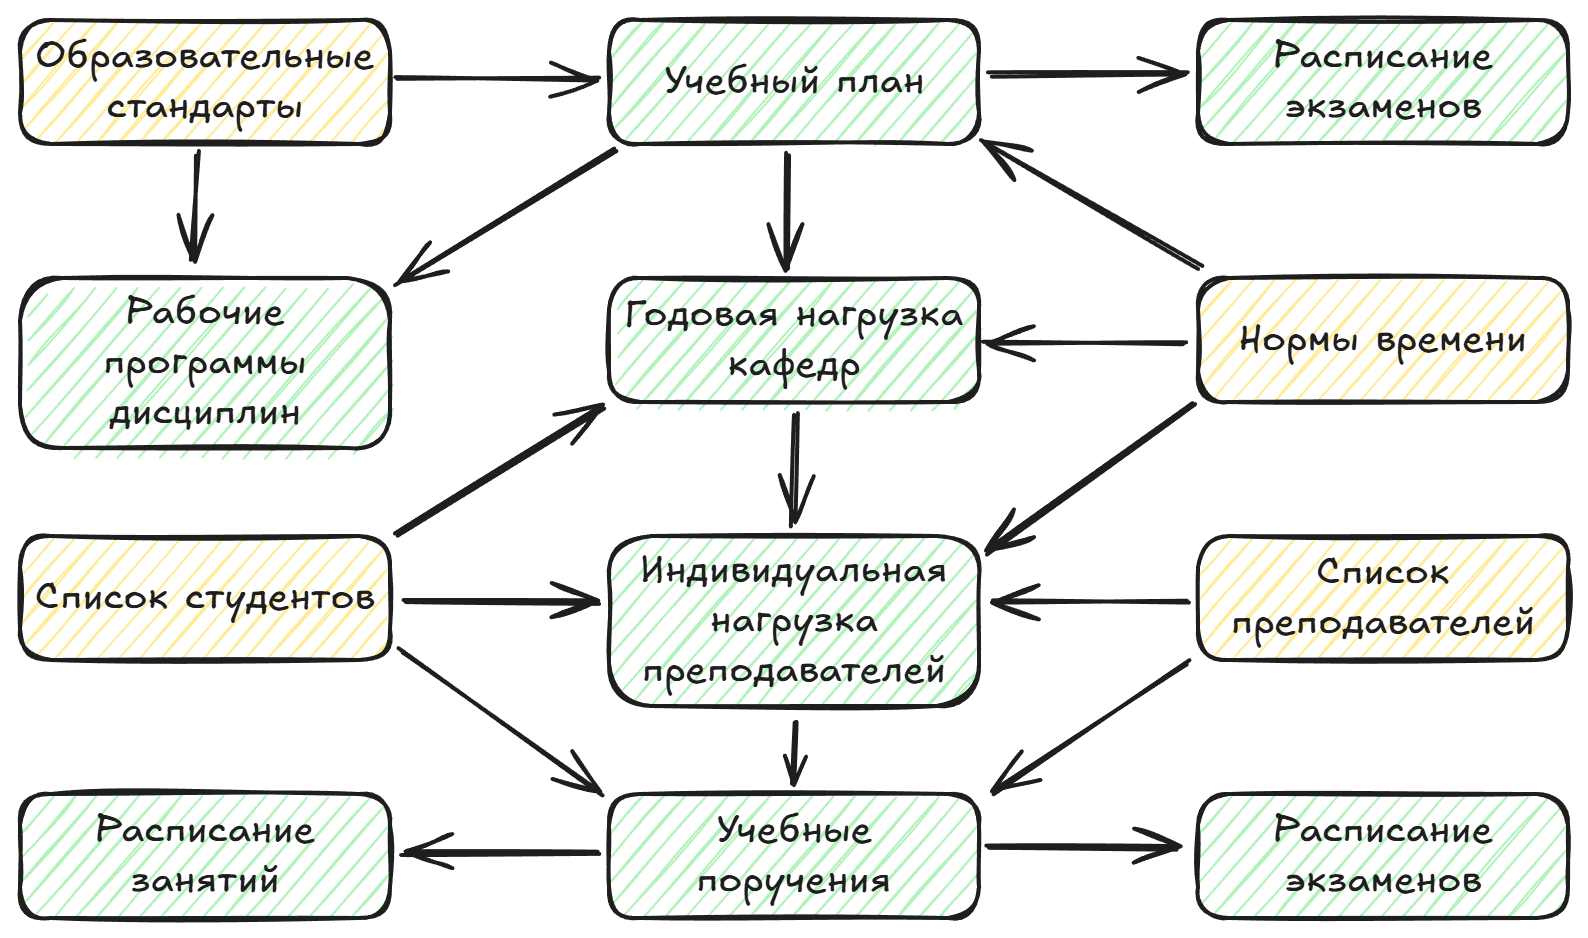
\includegraphics[width=1\textwidth]{images/ch2/docs.png}
	\caption{Диаграмма документов и таблиц управления учебным процессом}
	\label{fig:docs}
\end{figure}

Список студентов будет делиться на направления, согласно учебным планам, а также на группы и подгруппы для проведения семинаров и лабораторных занятий соответственно. Следует подметить, что деление на подгруппы является рудиментарным процессом, изначальный смысл которого заключался в невозможности вместить достаточное количество студентов в классы с компьютерами.

Не менее важным является подбор аудиторий для проведения учебных занятий. Главным параметром каждой аудитории является вместимость --- нельзя назначать учебное занятие в аудиторию, которая физически не может вместить весь контингент студентов и преподавателей на данное учебное занятие. Дополнительным, не менее важным параметром является требуемое оборудование для проведения учебного занятия: мультимедийное и лабораторное оборудование.

Схематичное дробление контингента студентов и здания вуза предоставлено на рисунке ниже (см. \figref{fig:fragmentation}).

\begin{figure}[H]
	\centering
	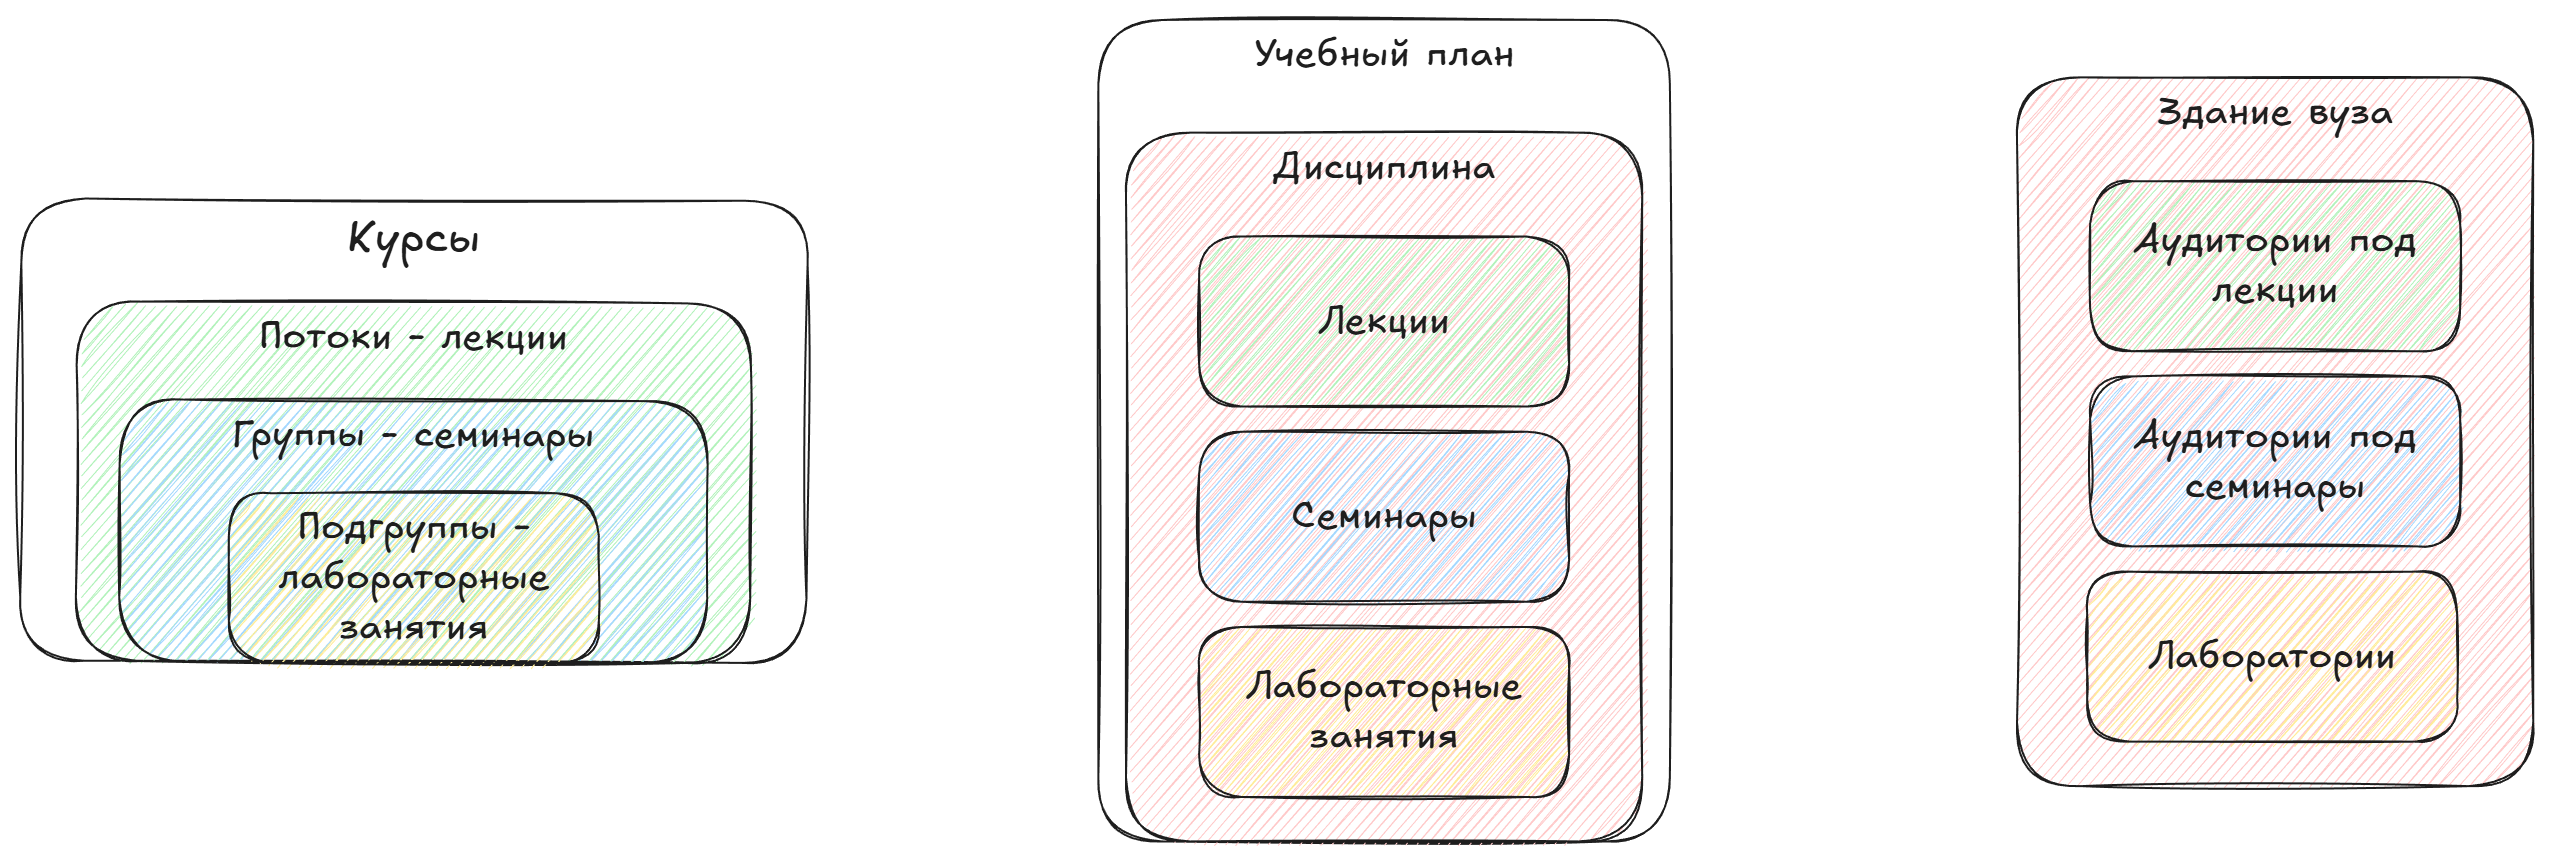
\includegraphics[width=1\textwidth]{images/ch2/fragmentation.png}
	\caption{Схематичное дробление контингента и здания вуза}
	\label{fig:fragmentation}
\end{figure}

\subsection{Допустимое решение}

\subsubsection{Коллапс волновой функции}

 WFC \cite{alonecoder:wavecollapse}, вдохновлённый редукцией фон Неймана. Название алгоритма произошло от физического процесса, при котором волновая функция, описывающая вероятностное состояние квантовой системы, при измерении переходит из суперпозиции возможных состояний в одной конкретное наблюдаемое состояние.

 В контексте задачи с составлением расписания её можно представить как суперпозицию здания университета. В каждой аудитории на каждый момент времени семестра существуют все возможные (удовлетворяющие ограничениям) учебные занятия конкретных групп и студентов. Для каждой такой ячейки высчитывается мера неопределённости --- энтропия, то есть количество возможных состояний. Далее ячейки с наименьшей энтропией коллапсируют в конкретные состояния из набора возможных, при этом учитывается вес состояния. Весом выступает функция полезности, как например большие веса в начале дня для групп на дневном обучении, и наоборот для групп на вечернем обучении. Именно гибкость этой функции позволяет модифицировать алгоритм решения под конкретные особенности того или иного образовательного учреждения. Коллапс волновой функции позволит найти приемлемое решение, то есть то, которое соответствует всем ограничениям, но в силу своей вероятностной природы решение не гарантирует глобального оптимума. Для того чтобы приблизить решение к глобальному оптимуму потребуется дополнительный шаг --- генетический алгоритм.

 \paragraph{Разрешение противоречий в WFC}

 Если в какой-то момент у всех доступных ячеек не остаётся допустимых вариантов коллапса, возникает противоречие.

 Для решения таких ситуаций в работе рассматриваются четыре подхода:
 \begin{itemize}
 	\item backtracking;
 	\item backjumping;
 	\item block based method;
 	\item полный перезапуск с нуля.
 \end{itemize}

 Backtracking. Метод backtracking является классическим способом устранения противоречий в задачах поиска с ограничениями.
 Если после очередного выбора система приходит к неразрешимому состоянию, алгоритм возвращается к предыдущему шагу, отменяет последнее решение и пробует следующий вариант.

 Формально процесс можно описать последовательностью решений \formref{eq:backtrack-seq}:
 \begin{equation}
 	S = \{s_1, s_2, \dots, s_k\},
 	\label{eq:backtrack-seq}
 \end{equation}
 \formwhere{где $S$~--- последовательность принятых решений;
 	\formwherenext{$s_i$}{решение на шаге $i$};
 	\formwherenext{$k$}{номер текущего шага}.}
 Каждое решение влияет на множество допустимых значений для следующих ячеек.
 При обнаружении противоречия выполняется откат \formref{eq:backtrack-rollback}:
 \begin{equation}
 	S \leftarrow \{s_1, s_2, \dots, s_{k-1}\}.
 	\label{eq:backtrack-rollback}
 \end{equation}
 \formwhere{где $\leftarrow$~--- возврат к предыдущему состоянию последовательности;
 	\formwherenext{$k-1$}{индекс шага, на который выполняется откат}.}

 Преимущество backtracking заключается в том, что он позволяет сохранить уже построенную часть расписания и использовать её повторно.
 Это особенно важно в задачах, где большая часть размещённых занятий остаётся корректной, а конфликт возникает только в локальной области.

 Однако у метода есть существенный недостаток: при большом числе ограничений количество возвратов может быстро расти.
 В задаче составления расписания это означает, что алгоритм может многократно пересчитывать одни и те же фрагменты, особенно если противоречие вызвано неудачным ранним выбором.

 Backjumping. Backjumping является расширением backtracking.
 Вместо возврата к непосредственно предыдущему решению алгоритм анализирует причину противоречия и откатывается не на один шаг, а к наиболее раннему решению, которое действительно повлияло на возникновение ошибки.

 Идея метода особенно полезна в расписаниях, где конфликт часто связан не с последним назначением, а с более ранним выбором, например:
 \begin{itemize}
 	\item преподаватель уже оказался занят в нужное время;
 	\item аудитория была закреплена за другим занятием;
 	\item группа получила пересечение по нескольким предметам.
 \end{itemize}

 Если конфликт возник из-за решений $s_i, s_j, s_k$, то backjumping позволяет перейти не к $s_{k-1}$, а сразу к наиболее релевантному из них.
 Это сокращает число бесполезных откатов и уменьшает время поиска.

 В практическом применении к расписанию метод backjumping полезен тогда, когда система хранит информацию о причинах исключения вариантов.
 Например, при удалении варианта можно фиксировать, какие уже назначенные занятия сделали его невозможным.
 Тогда при противоречии можно определить, какой именно шаг следует пересмотреть.

 Недостаток метода состоит в том, что для его эффективной работы требуется дополнительный учёт причин конфликтов, а это усложняет реализацию.

 Block based method. Block based method основан на локализации проблемы внутри части пространства поиска.
 Вместо пересчёта всей модели алгоритм выделяет блок --- набор связанных ячеек, внутри которого возникло противоречие, и пытается восстановить только этот фрагмент.

 Для задачи расписания блоком может быть:
 \begin{itemize}
 	\item одна учебная неделя;
 	\item один день;
 	\item конкретная пара групп, преподавателей и аудиторий.
 \end{itemize}

 Преимущество такого подхода состоит в том, что большая часть уже построенного расписания сохраняется.
 Это особенно удобно, если противоречие локализуется в ограниченной области и не затрагивает всю структуру решения.

 Принцип работы можно описать следующим образом:
 \begin{enumerate}
 	\item выделяется блок, в котором обнаружено противоречие;
 	\item внутри блока восстанавливается множество допустимых вариантов;
 	\item выполняется повторный коллапс только для этого блока;
 	\item если блок снова приводит к конфликту, он расширяется или пересобирается заново.
 \end{enumerate}

 В рамках расписания такой подход уменьшает число глобальных перезапусков, но требует аккуратного определения границ блока.
 Если блок выбран слишком маленьким, противоречие может просто переместиться в соседнюю область; если слишком большим --- метод теряет локальные преимущества.

 Начать всё заново. Подход полного перезапуска предполагает, что при обнаружении тупика алгоритм сбрасывает текущее состояние и строит решение заново.
 В WFC это означает удаление всей текущей частичной раскладки и повторный запуск процесса коллапса с новыми случайными выборами.

 Для задачи составления расписания такой подход особенно оправдан, потому что качественное решение часто зависит от ранних случайных выборов.
 Если эти выборы оказались неудачными, дальнейшее локальное исправление может быть неэффективным.
 В этом случае проще и быстрее полностью перезапустить алгоритм и получить новую траекторию поиска.

Именно этот подход был выбран в реализации алгоритма WFC для генерации расписания ВУЗа, так как он является очень простым в реализации и на удивление эффективным.

 \subsubsection{Satisfiability solvers}

 Satisfiability solvers (SAT solvers) --- это программы, решающие задачи булевой выполнимости
 (Boolean Satisfiability Problem).

 Основным вопросом SAT-задачи является: «можно ли подобрать значения true/false для переменных так, чтобы логическое выражение стало истинным?»

 Например, задана булева формула \formref{eq:sat-formula}:
 \begin{equation}
 	(A \lor B) \land (\neg A \lor C)
 	\label{eq:sat-formula}
 \end{equation}
 \formwhere{где $A$, $B$, $C$~--- булевы переменные.}

 SAT solver пытается найти такие значения переменных \formref{eq:sat-values}:
 \begin{equation}
 	A = \mathrm{false},\quad B = \mathrm{true},\quad C = \mathrm{true}
 	\label{eq:sat-values}
 \end{equation}
 \formwhere{где $\mathrm{false}$ и $\mathrm{true}$~--- логические значения «ложь» и «истина».}

 при которых вся формула становится истинной.

 Если такого набора не существует, solver доказывает, что формула
 невыполнима.

 \paragraph{Satisfiability Modulo Theories}

 Классический SAT solver работает только с булевой логикой, однако реальные задачи часто требуют работы с числами, массивами, строками и битовыми операциями.

 Для этого используются SMT solver'ы (Satisfiability Modulo Theories) \cite{z3:github}.

 Например, SMT solver способен анализировать систему ограничений \formref{eq:smt-x}--\formref{eq:smt-y-max}:
 \begin{equation}
 	x > 10
 	\label{eq:smt-x}
 \end{equation}
 \begin{equation}
 	y = x + 2
 	\label{eq:smt-y-def}
 \end{equation}
 \begin{equation}
 	y < 5
 	\label{eq:smt-y-max}
 \end{equation}
 \formwhere{где $x$, $y$~--- целочисленные переменные;
 	\formwherenext{$10$, $2$, $5$}{числовые константы в ограничениях}.}

 и определить, что такая система противоречива.

 \paragraph{Принцип работы}

 SAT/SMT solver --- это механизм поиска значений, удовлетворяющих набору ограничений.

 Вместо ручного перебора вариантов программист описывает:

 \begin{itemize}
 	\item переменные;
 	\item ограничения;
 	\item условия задачи.
 \end{itemize}

 После этого solver самостоятельно ищет решение или доказывает, что решения не существует. Такая программа может быть полезной при формировании учебных планов, чтобы удостовериться, что план не будет нарушать жёсткие ограничения.

 SMT-solver также может выступать в роли алгоритма формирования приемлемого решения, однако его природа заключается в том, чтобы найти любое решение но быстро. WFC же в то время сможет не просто найти случайное решение, но и уже на этом этапе применить ряд оптимизаций решения.

\subsection{Оценка решения}

После получения первичного решения, которое удовлетворяет всем обязательным требованиям требуется провести итеративный процесс улучшения этого расписания. Для того, чтобы что-либо улучшать, нужно уметь давать оценку полученным результатам.

Самым важным критерием оценки является соответствие минимальным требованиям:

\begin{itemize}
	\item все учебные занятия согласно учебному плану \cite{stankin:edu_programs};
	\item весь учебный процесс проходит в период согласно календарному учебному графику \cite{stankin:calendar};
	\item не нарушаются нормы времени;
	\item учебные занятия должны начинаться в строго отведённое под них время с 8:30 утра, по 22:50, без учёта выходных дней и праздников \cite{tkrf:112}.
\end{itemize}

Для оценки будет рассчитываться множество различных параметров. Одним из самых главных таких параметров является непрерывность расписания --- в прекрасном расписании будущего не должно быть «окон», на которых студенты имеют свойство расходится по домам.

Ещё один важный параметр --- это равномерность расписания. Не должно быть расписания, где в понедельник пять пар, а во вторник только одна. Согласно исследованию, проведённому Клеванским Николаем Николаевичем \cite{klivansky:forming_schedule} студенты предпочитают, когда одни и те же пары проводятся в одно и то же время в разные дни недели. Соответственно существует три оценки равномерности:

\begin{itemize}
	\item равномерность загруженности;
	\item равномерность начала занятий;
	\item равномерность идентичности пар по дням / неделям.
\end{itemize}

Дополнительным параметром может являться «компоновка» ВУЗа. Для экономии временных и финансовых ресурсов можно попробовать уместить весь учебный процесс в меньший набор аудиторий. Также можно пробовать уменьшать среднюю дистанцию, требуемую для перехода из одной аудитории в другую между учебными занятиями. В случае проведения лабораторных занятий дистанционно можно не делить на подгруппы, начинать семинары только после лекций по каждой дисциплине и т. д.

\subsection{Оптимизация решения}

\subsubsection{Генетический алгоритм}

Генетический алгоритм представляет собой эвристический метод поиска оптимального решения,
механизм работы которого аналогичен процессу естественного отбора в природе. В рамках данной задачи
в качестве генома рассматривается полное расписание учебного заведения на семестр.

В научной литературе уже были упомянуты комбинации алгоритма WFC с генетическим алгоритмом \cite{bailly:geneticwfc}, однако этот подход не применялся к задачам составления расписания.

Хромосома кодирует расписание на один семестр и состоит из набора генов, где каждый ген
соответствует конкретному элементу расписания.
Размер хромосомы определяется \formref{eq:chromosome-size}:
\begin{equation}
	|H| = n \times 6 \times 182{,}625,
	\label{eq:chromosome-size}
\end{equation}
\formwhere{где $|H|$~--- размер хромосомы;
	\formwherenext{$n$}{количество учебных групп};
	\formwherenext{$6$}{количество учебных дней в неделю};
	\formwherenext{$182{,}625$}{усреднённое количество учебных дней в семестре (варьируется каждый семестр)}.}

Операторы мутации реализуются с использованием локальных методов поиска, например алгоритма имитации отжига, что позволяет эффективно исследовать окрестность текущего решения и избегать застревания в локальных минимумах.

\subsubsection{Имитация отжига}

Имитация отжига (SA) представляет собой стохастический метод локального поиска, основанный на аналогии с физическим процессом охлаждения твёрдых тел, при котором система постепенно переходит к состоянию с минимальной энергией. В контексте задачи оптимизации расписания данный алгоритм используется для улучшения текущего решения путём итерационного поиска его окрестностей (см. \figref{fig:sa}).

\begin{figure}[H]
	\centering
	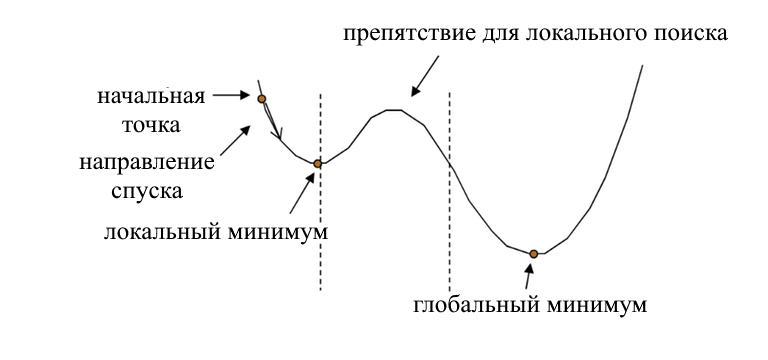
\includegraphics[width=0.9\textwidth]{images/ch2/sa.png}
	\caption{Проблематика локальных методов поиска}
	\label{fig:sa}
\end{figure}

На каждой итерации из текущего решения формируется новое, соседнее решение путём небольшого случайного
изменения (например, перестановки занятий в расписании). Если новое решение имеет более высокое значение целевой функции, оно принимается. В противном случае оно может быть принято с некоторой вероятностью, определяемой \formref{eq:sa-accept}:
\begin{equation}
	P = \exp\left(-\frac{\Delta E}{T}\right),
	\label{eq:sa-accept}
\end{equation}
\formwhere{где $P$~--- вероятность принятия ухудшающего решения;
	\formwherenext{$T$}{параметр температуры алгоритма};
	\formwherenext{$\Delta E$}{ухудшение значения функции приспособленности}.}

Параметр температуры постепенно уменьшается согласно заданному расписанию охлаждения, что приводит к снижению вероятности принятия ухудшающих решений и обеспечивает сходимость алгоритма к локально оптимальному решению.

\subsection{Вывод по второй главе}

Предложенный гибридный подход, основанный на применении алгоритма коллапса волновой
функции и последующей оптимизации с помощью генетического алгоритма, позволяют решать задачу
составления расписания, при этом поддерживая достаточную гибкость для адаптации к различным
образовательным учреждениям.

	\FloatBarrier

	%Глава3
	\FloatBarrier
	\clearpage
	\newpage
	\pagestyle{fancy}
	\section{Разработка архитектуры будущего программного продукта}


	%Глава4
	\FloatBarrier
	\clearpage
	\newpage
	\pagestyle{fancy}
	\section{Выбор средств реализации сервиса для программной поддержки генерации расписания учебных заведений}

\subsection{Обоснование выбора СУБД}

При выборе СУБД требуется учесть главные факторы:

\begin{itemize}
	\item размер данных: для генерации расписания не требуется огромный объём данных. Учебные планы, списки групп, списки преподавателей и т. д. занимают относительно небольшое место на диске;
	\item тип данных: данные для генерации расписаний являются текстовыми данными и легко могут храниться в любой СУБД или даже просто в текстовом файле, как JSON или CSV;
	\item требование к производительности: нагрузка на базу данных будет минимальная – генерировать расписание не требуется чаще, чем раз в семестр;
	\item простота использования: главной задачей ВКР является сам алгоритм генерации расписания, база данных является лишь второстепенной задачей, которая не должна отнимать много времени на развёртывание и заполнение.
\end{itemize}

Учитывая вышеперечисленные факторы, можно прийти к выводу, что для поставленной задачи требуется небольшая, легковесная база данных.

\subsubsection{Хранение данных в текстовых файлах}

Хранения данных в текстовых файлах, таких как JSON, TXT или CSV отлично подходит для поставленной задачи. Из плюсов можно выделить простоту использования, подходит для хранения сложных, вложенных структур данных, легко читается человеком и легко вносить изменения в структуру данных.

Однако есть и минусы. При каждом чтении будет производится операция парсинга текстовых данных, что будет делать операции чтения, изменения или добавления сравнительно медленными. Более того, такие, классические для СУБД вещи как поиск, индексация, транзакции отсутствуют, а сами данные будут храниться не в бинарном файле, а в текстовом, что будет неоправданно раздувать объём хранимых данных.

Текстовый формат данных отлично подходит для транспортировки небольших объёмов данных, таких как уже сгенерированное расписание, на клиент для дальнейшего отображения расписания учебных занятий. Однако текстовые файлы не идеально подходят для хранения и работы с данными, используемыми в процессе генерации расписания.

\subsubsection{SQLite}

SQLite – это самодостаточная и встроенная СУБД. Для развёртывания которой не требуется сервер или сложная система управления. Все данные хранятся в бинарном файле прямо в проекте с расширением “.sqlite” или “.db”.

Из минусов часто выделяют ограничение по объёму данных до 140Тб, однако это не будет проблемой для хранения данных для генерации расписаний учебных занятий. Также SQLite не подходит для сложных многопользовательских сценариев – отсутствует полноценная поддержка конкурентности.

\subsubsection{Вывод}

При небольшом анализе вариантов СУБД для хранения данных проекта выбор пал на SQLite. Это легковесная СУБД, обладающая всеми преимуществами классических СУБД как индексация и скорость обработки запросов, но и в то же время обладающая всеми преимуществами хранения данных в текстовых файлах – простота и гибкость. Более того, у автора данной выпускной квалификационной работы уже был опыт работы с SQLite, а соответственно не будет проблем с использованием, связанных с низким уровнем компетенции в инструменте.

\subsection{Выбор средств реализации сервера}

\subsection{Выбор средств реализации клиента}

\subsection{Вывод по четвёртой главе}

Был произведён сравнительный анализ подходящих для проекта СУБД и сделан обоснованный выбор на SQLite. 
	\FloatBarrier

	%Глава 5
	\FloatBarrier
	\clearpage
	\newpage
	\pagestyle{fancy}
	\section{Реализация  сервиса для программной поддержки генерации расписания учебных заведений}

\subsection{Заполнение базы данных}

В идеальном сценарии для заполнения базы данных можно использовать API систем университета, хранящих такие данные как списки групп, преподавателей и учебные планы. Однако на момент написания данной выпускной квалификационной работы такая возможность отсутствует.

Альтернативный вариант – производить парсинг PDF файлов учебных планов и календарных учебных графиков, которые находятся в открытом доступе на сайте университета \cite{stankin:edu_programs} \cite{stankin:calendar}.

Однако существует третий вариант: переиспользовать написанный автором данной выпускной квалификационно работы в бакалавриате парсер \cite{github:grad_work_alpha} PDF файлов расписаний учебных занятий. Хоть это и не будет финальным решением, готовым для запуска системы в работу на пользу учебного заведения – это будет путём наименьшего сопротивления.

Этот подход также решит две другие проблемы, не имеющие элегантного решения. Тогда, как списки групп можно получить из соответствующего форума в ЭОС ФГБОУ ВО «МГТУ «СТАНКИН» \cite{stankin:groups}, актуальные списки преподавательского состава или таблицы со всеми учебными аудиториями и оборудованием найти не получится. В случае получения данных сразу из готового расписания за прошлый семестр можно определить и какие предметы ведут какие преподаватели, и какие предметы проводятся в каких аудиториях.

\subsubsection{Процесс популяции базы данных}

Скачать все расписания на текущий семестр можно в соответствующем форуме в ЭОС ФГБОУ ВО «МГТУ «СТАНКИН» \cite{stankin:schedule}.

Для заполнения базы данных требуемыми данными была написана специальная вспомогательная программа \cite{github:subject_parser}, производящая парсинг данных и приводящая их в нужную структуру и формат в SQLite (см. Рис.~\ref{fig:db}).

\begin{figure}[H]
	\centering
	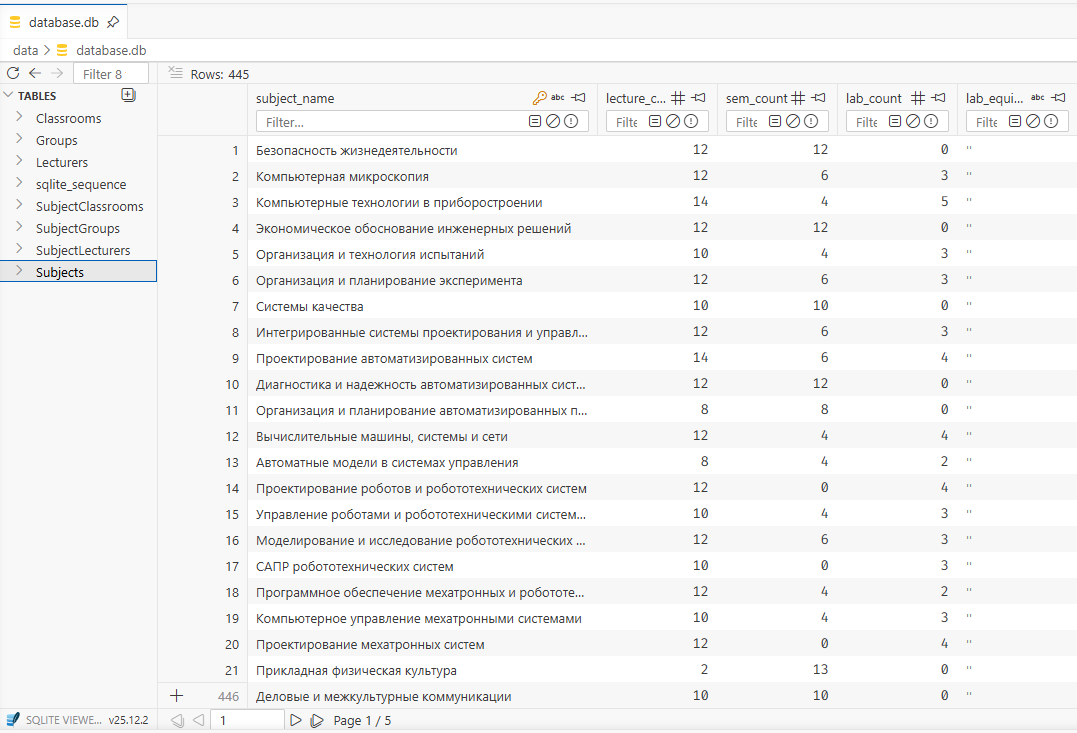
\includegraphics[width=1\textwidth]{images/ch5/db.png}
	\caption{Заполненная БД}
	\label{fig:db}
\end{figure}

\subsection{Сервер}

Как уже описывалось в предыдущей главе, в качестве основы вычислительной части проекта был выбран Polars. На основе его декларативного языка программирования был реализован алгоритм решения задачи.
Все основные методы были обёрнуты в REST API благодаря FastAPI, а Swagger позволил упростить процесс написания будущего клиента.

Также были разработаны дополнительные инструменты визуализации расписания для упрощения дебага текущего состояния расписания, как например интерактивная визуализация всего расписания на семестр (см. Рис.~\ref{fig:debug}).

\begin{figure}[H]
	\centering
	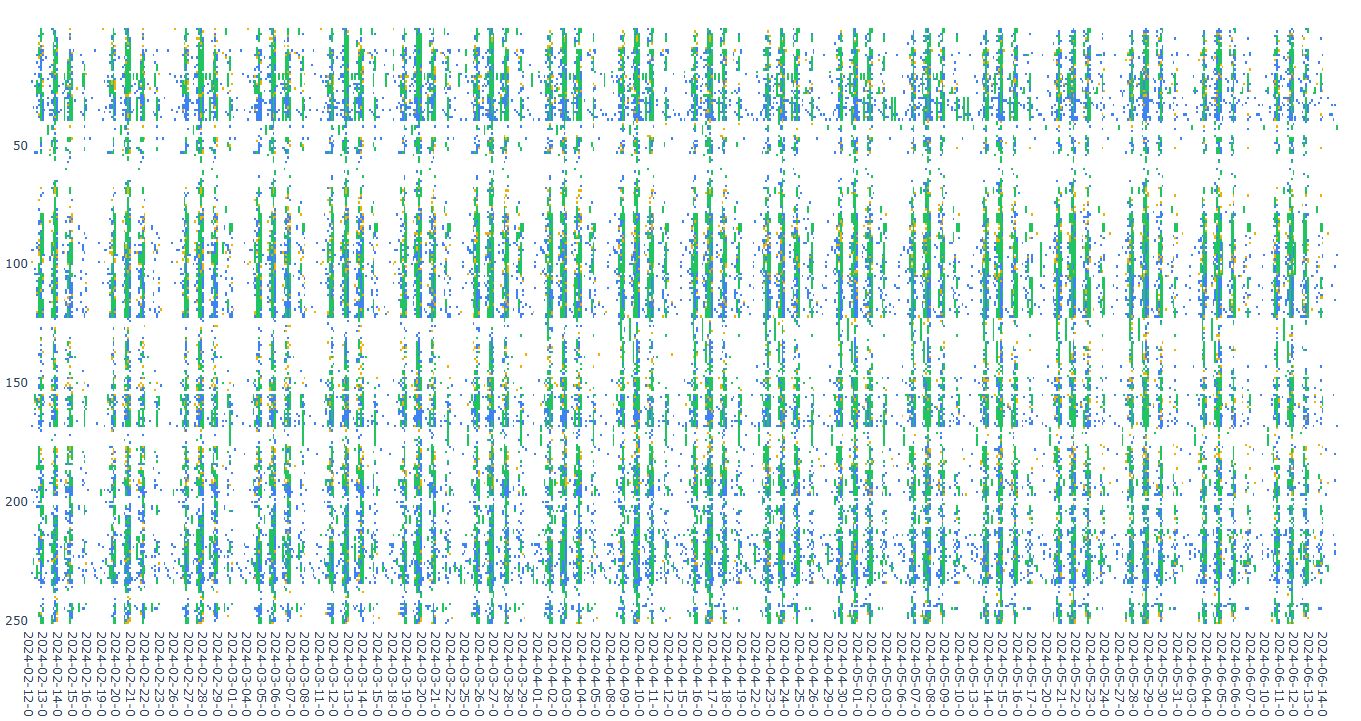
\includegraphics[width=1\textwidth]{images/ch5/debug.png}
	\caption{Интерактивная визуализация расписания университета на семестр}
	\label{fig:debug}
\end{figure}

\subsection{Клиент}

В роли клиента было написано веб-приложение на базе Nuxt 4 и Vue 3.5 (см. Рис.~\ref{fig:client}), а технология progressive web application (PWA) позволяет установить сайт как нативное приложения на любое современное устройство, поддерживающие браузер. То есть генерацию расписания можно производить даже с некоторых холодильников или наручных часов.

\begin{figure}[H]
	\centering
	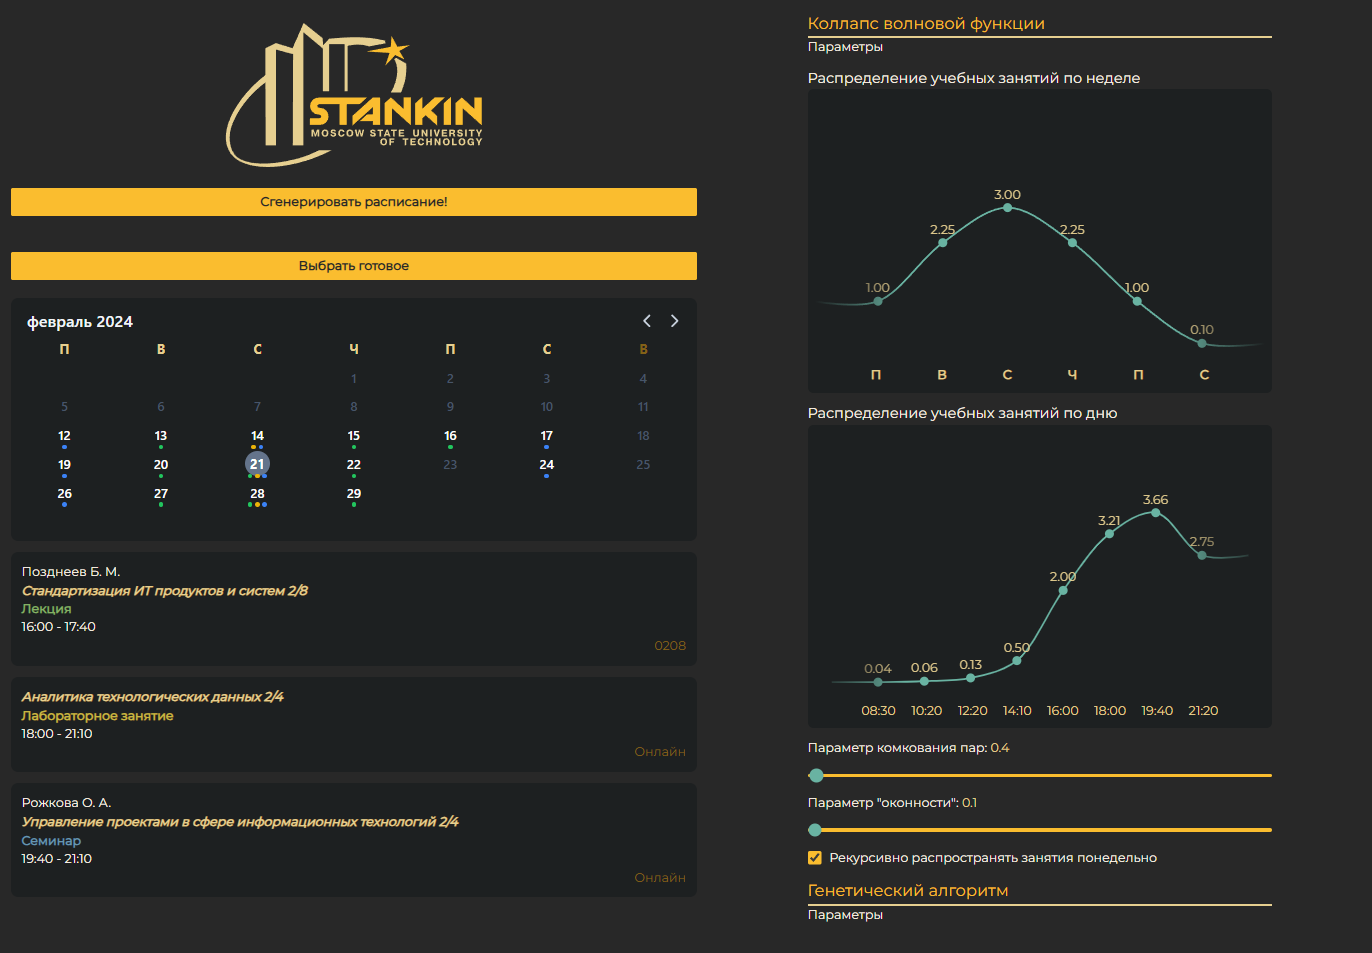
\includegraphics[width=1\textwidth]{images/ch5/client.png}
	\caption{Клиент}
	\label{fig:client}
\end{figure}

\subsection{Вывод по пятой главе}

Была реализована программная основа сервиса для генерации расписания учебных занятий. Для системы была реализована трёхзвенная архитектура, обеспечивающая разделение ответственности между хранилищем данных, серверной логикой и пользовательским интерфейсом. Был подготовлен механизм заполнения БД на основе доступных источников данных.

На стороне сервера реализована бизнес-логика и REST API для взаимодействия с клиентской частью и внешними компонентами системы. На стороне клиента разработано веб-приложение, позволяющее удобно работать с сервисом через браузер. В результате получена работоспособная система, пригодная для дальнейшего развития и последующей интеграции в более полный процесс автоматизированного формирования расписания.

	\FloatBarrier

	%Глава 6
	\FloatBarrier
	\clearpage
	\newpage
	\pagestyle{fancy}
	\section{Руководство пользователя}

Данная глава находиться в активной разработке.

	\FloatBarrier

	%Глава 7
	\FloatBarrier
	\clearpage
	\newpage
	\pagestyle{fancy}
	\section{Экономическое обоснование}

Актуальность автоматизации процесса составления расписания подтверждается не только внутренними затратами учебного заведения, но и запросом студенческого сообщества. Во «ВКонтакте» размещена петиция «Расписание за неделю» \cite{vk:schedule_petition}, в которой обучающиеся МГТУ «СТАНКИН» фиксируют потребность в своевременной и полной публикации расписания занятий на неделю вперёд, а не фрагментарном или запоздалом доведении информации до студентов и преподавателей. Подобные обращения свидетельствуют о том, что качество и оперативность расписания напрямую влияют на удовлетворённость участников образовательного процесса и воспринимаются как значимый фактор организации учебной деятельности вуза.

С экономической точки зрения такой запрос означает необходимость сократить цикл подготовки и пересборки расписания, снизить число ошибок при ручном согласовании и обеспечить единый канал публикации результата. Разрабатываемое программное средство направлено на устранение этих проблем и тем самым отвечает как организационным потребностям УМУ, так и ожиданиям контингента, выраженным в публичной инициативе.

\subsection{Анализ аналогов и обоснование собственного решения}

Для оценки целесообразности разработки и внедрения программного средства поддержки генерации расписания учебных занятий необходимо рассмотреть существующие подходы к решению данной задачи в образовательных организациях.

В МГТУ «СТАНКИН» на момент выполнения выпускной квалификационной работы расписание на семестр формируется вручную сотрудниками УМУ \cite{stankin:schedule}. Данный процесс является базовым аналогом: он не требует лицензий на программное обеспечение, но связан с высокими трудозатратами, риском ошибок при согласовании ограничений и длительным циклом пересборки расписания при изменении исходных данных.

На российском рынке представлены специализированные системы автоматизированного составления расписания для вузов.

\textbf{Галактика РУЗ} \cite{galaktika:ruz} --- комплексное решение для управления учебным процессом в высших учебных заведениях. Система поддерживает автоматическое формирование опорного расписания, контроль параметризуемых ограничений, публикацию результатов на сайте вуза и в мобильных приложениях. Внедрение предполагает закупку лицензий и сопутствующей инфраструктуры.

\textbf{1С:Автоматизированное составление расписания. Университет} \cite{1c:schedule} --- продукт экосистемы 1С для автоматизированного, ручного и смешанного составления расписаний с учётом нагрузки преподавателей, аудиторного фонда и учебных планов. Типовое внедрение включает лицензирование, настройку под регламенты вуза и интеграцию с другими модулями 1С.

\textbf{ТАНДЕМ.Университет} (модуль «Расписание») \cite{tandem:schedule} --- модуль корпоративной системы управления вузом. Обеспечивает автоматическое и ручное составление расписания, фиксацию ограничений преподавателей и требований к аудиториям, поддержку индивидуальных образовательных траекторий.

\textbf{Экспресс-расписание ВУЗ} \cite{express:schedule} --- программа для автоматического составления расписания в локальной или сетевой конфигурации. Поддерживает работу с подгруппами, планирование отсутствия преподавателей и публикацию расписания на сайте образовательной организации.

Зарубежные системы \textbf{UniTime} и \textbf{TimeEdit}, широко применяемые в зарубежных вузах, рассматриваются в обзорной литературе по задаче составления расписаний \cite{vrielink:patat2016}, однако их внедрение в российский вуз сопряжено с адаптацией нормативной базы, локализацией и интеграцией с отечественными информационными системами.

Разрабатываемое в рамках данной выпускной квалификационной работы программное средство не претендует на полную замену корпоративных ERP-систем, но ориентировано на узкую задачу --- генерацию и оптимизацию расписания с учётом правил МГТУ «СТАНКИН», предпочтений преподавателей, «компоновки вуза» и публикации результата через веб-интерфейс и PWA-клиент. Использование открытого программного стека (Python, FastAPI, Polars, SQLite, Nuxt) снижает стоимость владения по сравнению с коммерческими аналогами.

На основе описания функциональности перечисленных решений проведён сравнительный анализ (см. \tabref{tab:analogs}).

\begin{table}[H]
	\centering
	\caption{Сравнительная таблица функций аналогов и целевого программного продукта}
	\label{tab:analogs}
	\begin{tabularx}{\textwidth}{|>{\raggedright\arraybackslash}X|>{\centering\arraybackslash}p{2.3cm}|>{\centering\arraybackslash}p{2.5cm}|>{\centering\arraybackslash}p{2.5cm}|}
		\hline
		\textbf{Критерий} &
		\textbf{Ручной процесс} &
		\textbf{Коммерч.\ системы} &
		\textbf{Продукт ВКР} \\
		\hline
		Автогенерация с учётом нормативов & $-$ & $+$ & $+$ \\
		\hline
		Учёт предпочтений преподавателей & $\pm$ & $+$ & $+$ \\
		\hline
		Оптимизация перемещений (компоновка) & $-$ & $\pm$ & $+$ \\
		\hline
		Адаптация под правила вуза & $+$ & $\pm$ & $+$ \\
		\hline
		Низкая стоимость владения & $+$ & $-$ & $+$ \\
		\hline
		Веб-доступ и PWA & $\pm$ & $+$ & $+$ \\
		\hline
	\end{tabularx}
\end{table}

Целевой программный продукт превосходит ручной процесс по скорости пересборки расписания и снижению числа конфликтов ограничений. По сравнению с коммерческими ERP-модулями он обеспечивает специализацию под регламенты МГТУ «СТАНКИН» и контролируемую совокупную стоимость владения за счёт открытого программного обеспечения. Таким образом, разработка собственного решения экономически оправдана как альтернатива как полностью ручному составлению, так и закупке дорогостоящего типового продукта без гарантии покрытия всех специфических требований вуза.

\subsection{Оценка затрат проекта}

Для оценки затрат на создание и внедрение программного средства определены следующие ключевые ресурсы:

\begin{itemize}
	\item разработчик (full-stack, автор ВКР) --- проектирование, реализация серверной и клиентской частей, алгоритмов генерации;
	\item специалист по внедрению и сопровождению (системный администратор) --- развёртывание в контуре вуза, обучение пользователей, техническая поддержка;
	\item программное обеспечение --- операционная система, среда разработки, серверные компоненты;
	\item инфраструктура и оборудование --- сервер приложений и рабочее место администратора.
\end{itemize}

Затраты на разработку оцениваются ретроспективно по этапам, отражённым в главах~3--5 выпускной квалификационной работы, с учётом доработок после защиты. Затраты на внедрение и эксплуатацию относятся к первому году использования системы в МГТУ «СТАНКИН».

Для расчёта приняты следующие ставки оплаты труда: разработчик --- 1000~руб./ч, системный администратор --- 500~руб./ч

Расчёт прямых трудозатрат приведён в \tabref{tab:labor}.

\begin{table}[H]
	\centering
	\caption{Расчёт прямых трудозатрат}
	\label{tab:labor}
	\begin{tabularx}{\textwidth}{|>{\raggedright\arraybackslash}X|r|>{\raggedright\arraybackslash}p{2.6cm}|r|}
		\hline
		\textbf{Наименование работ} &
		\textbf{Часы} &
		\textbf{Специалист} &
		\textbf{Затраты, руб.} \\
		\hline
		Проектирование архитектуры и БД (гл.~3) & 80 & Разработчик & 80\,000 \\
		\hline
		Выбор и настройка стека (гл.~4) & 40 & Разработчик & 40\,000 \\
		\hline
		Парсер и наполнение БД (гл.~5) & 60 & Разработчик & 60\,000 \\
		\hline
		Сервер: WFC, оптимизация, API (гл.~5) & 140 & Разработчик & 140\,000 \\
		\hline
		Клиент Nuxt, PWA (гл.~5) & 80 & Разработчик & 80\,000 \\
		\hline
		Тестирование и отладка (гл.~5) & 60 & Разработчик & 60\,000 \\
		\hline
		Доработки после защиты ВКР & 40 & Разработчик & 40\,000 \\
		\hline
		\textbf{Итого разработка} & \textbf{500} & & \textbf{500\,000} \\
		\hline
		Развёртывание в контуре вуза & 60 & Администратор & 30\,000 \\
		\hline
		Обучение сотрудников УМУ & 40 & Администратор & 20\,000 \\
		\hline
		Поддержка ($10$~ч/мес $\times 12$) & 120 & Администратор & 60\,000 \\
		\hline
		\textbf{Итого внедрение и эксплуатация} & \textbf{220} & & \textbf{110\,000} \\
		\hline
	\end{tabularx}
\end{table}

Общая сумма расходов на трудозатраты составляет 610\,000~руб., общая трудоёмкость --- 720~чел.-часов.

Основная часть программного обеспечения проекта распространяется бесплатно (см. \tabref{tab:software}), что соответствует выбранному в главе~4 стеку технологий.

\begin{table}[H]
	\centering
	\caption{Расчёт затрат на программное обеспечение}
	\label{tab:software}
	\begin{tabularx}{\textwidth}{|>{\raggedright\arraybackslash}X|r|>{\raggedright\arraybackslash}X|}
		\hline
		\textbf{Наименование} & \textbf{Стоимость, руб.} & \textbf{Примечание} \\
		\hline
		Python, FastAPI, Polars, SQLite & 0 & Открытый исходный код \\
		\hline
		Nuxt, Vue, TypeScript, pnpm & 0 & Открытый исходный код \\
		\hline
		Ubuntu Server, Git, VS Code & 0 & Бесплатное ПО \\
		\hline
		Лицензия на антивирус & 5\,000 & Стоимость на 1 год \\
		\hline
	\end{tabularx}
\end{table}

Для размещения серверной части и работы администратора необходимо серверное и клиентское оборудование (см. \tabref{tab:infra}). В отличие от типовых смет внедрения учётных систем, в проекте не закладывается лицензия Windows Server --- используется Linux.

\begin{table}[H]
	\centering
	\caption{Расчёт затрат на инфраструктуру}
	\label{tab:infra}
	\begin{tabularx}{\textwidth}{|>{\raggedright\arraybackslash}p{2.5cm}|>{\raggedright\arraybackslash}X|c|r|}
		\hline
		\textbf{Часть} & \textbf{Наименование} & \textbf{Кол-во, ед.} & \textbf{Стоимость, руб.} \\
		\hline
		Серверная & Сервер приложений (8 ядер, 32~ГБ ОЗУ, SSD) & 1 & 100\,000 \\
		\hline
		Клиентская & ПК администратора (16~ГБ ОЗУ) & 1 & 65\,000 \\
		\hline
		Серверная & Сетевое оборудование & 1 & 2\,000 \\
		\hline
		\multicolumn{3}{|r|}{\textbf{Итого}} & \textbf{167\,000} \\
		\hline
	\end{tabularx}
\end{table}

Амортизация оборудования рассчитывается линейным методом по \formref{eq:amort-year}. Срок полезного использования принят равным 7~годам:
\begin{equation}
	A_{\mathrm{год}} = \frac{C_{\mathrm{обор}}}{T_{\mathrm{сл}}},
	\label{eq:amort-year}
\end{equation}
\formwhere{где $A_{\mathrm{год}}$~--- годовая сумма амортизации, руб.;
	\formwherenext{$C_{\mathrm{обор}}$}{первоначальная стоимость оборудования, руб.};
	\formwherenext{$T_{\mathrm{сл}}$}{срок полезного использования, лет}.}

Годовая сумма амортизации составляет $167\,000 / 7 \approx 24\,000$~руб. Для периода внедрения в первый год (5~месяцев) в смету включена доля амортизации 15\,000~руб. (см. \tabref{tab:depreciation}).

\begin{table}[H]
	\centering
	\caption{Расчёт затрат на амортизацию (годовые показатели)}
	\label{tab:depreciation}
	\begin{tabularx}{\textwidth}{|>{\raggedright\arraybackslash}X|r|r|}
		\hline
		\textbf{Наименование} & \textbf{Стоимость, руб.} & \textbf{Амортизация в год, руб.} \\
		\hline
		Сервер приложений & 100\,000 & 14\,286 \\
		\hline
		ПК администратора & 65\,000 & 9\,286 \\
		\hline
		Сетевое оборудование & 2\,000 & 286 \\
		\hline
		\textbf{Итого} & \textbf{167\,000} & \textbf{24\,000} \\
		\hline
	\end{tabularx}
\end{table}

Затраты на электроэнергию за год оцениваются по \formref{eq:energy-cost}:
\begin{equation}
	Z_{\mathrm{эл}} = P \cdot t \cdot c,
	\label{eq:energy-cost}
\end{equation}
\formwhere{где $Z_{\mathrm{эл}}$~--- затраты на электроэнергию за год, руб.;
	\formwherenext{$P$}{потребляемая мощность, кВт};
	\formwherenext{$t$}{время работы оборудования в год, ч};
	\formwherenext{$c$}{тариф, руб./(кВт$\cdot$ч)}.}

Для сервера и рабочего места администратора суммарная мощность принята равной 0{,}5~кВт при 1600~ч работы в год и тарифе 5{,}47~руб./(кВт$\cdot$ч):
$Z_{\mathrm{эл}} = 0{,}5 \cdot 1600 \cdot 5{,}47 \approx 4\,400$~руб./год.

Затраты на ремонт и обслуживание оборудования оцениваются в 10\,\% от его стоимости в год: $167\,000 \cdot 0{,}1 = 16\,700$~руб.

Исходя из проведённых вычислений, сформирована общая смета затрат на первый год внедрения (см. \tabref{tab:budget}).

\begin{table}[H]
	\centering
	\caption{Общая смета затрат на проект (первый год)}
	\label{tab:budget}
	\begin{tabularx}{\textwidth}{|>{\raggedright\arraybackslash}X|r|}
		\hline
		\textbf{Статья затрат} & \textbf{Сумма, руб.} \\
		\hline
		Трудозатраты разработки (ВКР и доработки) & 500\,000 \\
		\hline
		Трудозатраты внедрения и поддержки & 110\,000 \\
		\hline
		Программное обеспечение & 5\,000 \\
		\hline
		Инфраструктура & 167\,000 \\
		\hline
		Амортизация (доля за период внедрения) & 15\,000 \\
		\hline
		Электроэнергия и ремонт & 21\,100 \\
		\hline
		\textbf{Итого} & \textbf{818\,100} \\
		\hline
	\end{tabularx}
\end{table}

\subsection{Обоснование экономической выгоды проекта}

Внедрение программного средства поддержки генерации расписания обеспечит следующие экономические преимущества для МГТУ «СТАНКИН»:

\begin{itemize}
	\item сокращение ручного труда сотрудников УМУ при пересборке расписания на семестр;
	\item снижение числа конфликтов по аудиториям, нагрузке преподавателей и «окнам» в расписании;
	\item ускорение публикации актуального расписания через веб-интерфейс и PWA вместо разрозненных файлов;
	\item учёт предпочтений преподавателей и оптимизация перемещений между корпусами без многократных ручных согласований.
\end{itemize}

Для количественной оценки эффекта используются допущения. Базовые трудозатраты УМУ на ручное составление расписания оцениваются так: 3~сотрудника $\times$ 120~ч $\times$ 500~руб./ч $=$ 180\,000~руб. за семестр, или 360\,000~руб. в год (два семестра).

Автоматизация позволяет сократить трудозатраты на подготовку и корректировку расписания на 35--40\,\%. При коэффициенте сокращения $k = 0{,}375$ годовая экономия определяется \formref{eq:year-savings}:
\begin{equation}
	E_{\mathrm{год}} = Z_{\mathrm{баз}} \cdot k = 360\,000 \cdot 0{,}375 = 135\,000~\text{руб.}
	\label{eq:year-savings}
\end{equation}
\formwhere{где $E_{\mathrm{год}}$~--- годовая экономия трудозатрат, руб.;
	\formwherenext{$Z_{\mathrm{баз}}$}{базовые годовые трудозатраты УМУ без автоматизации, руб.};
	\formwherenext{$k$}{коэффициент сокращения трудозатрат}.}

Сравнение с закупкой коммерческого решения для вуза сопоставимого масштаба (по аналогии с оценками внедрения типовых учётных систем) показывает, что совокупные затраты на лицензию, кастомизацию и внедрение могут составить 1{,}5--2{,}5~млн~руб. Разработка и внедрение собственного средства по смете \tabref{tab:budget} обходятся примерно в 818\,100~руб., то есть прямая экономия на капитальных затратах (CAPEX) по сравнению с коммерческим аналогом составляет порядка 0{,}7--1{,}7~млн~руб. при сопоставимом базовом функционале генерации расписания.

Срок окупаемости проекта по операционной экономии УМУ определяется \formref{eq:payback}:
\begin{equation}
	T_{\mathrm{ок}} = \frac{Z_{\mathrm{проект}}}{E_{\mathrm{год}}} = \frac{818\,100}{135\,000} \approx 6{,}1~\text{года}.
	\label{eq:payback}
\end{equation}
\formwhere{где $T_{\mathrm{ок}}$~--- срок окупаемости проекта, лет;
	\formwherenext{$Z_{\mathrm{проект}}$}{затраты на проект по смете, руб.};
	\formwherenext{$E_{\mathrm{год}}$}{годовая экономия трудозатрат, руб.}.}

При учёте отказа от закупки коммерческой лицензии совокупный экономический эффект превышает затраты на проект уже в первый год эксплуатации.

Дополнительно повышается качество расписания: уменьшение «окон», равномерность нагрузки и учёт «компоновки вуза» снижают косвенные потери времени студентов и преподавателей, не полностью отражённые в расчёте $E_{\mathrm{год}}$.

\subsection{Вывод по экономическому обоснованию}
Разработка и внедрение программного средства поддержки генерации расписания для МГТУ «СТАНКИН» экономически целесообразны как альтернатива полностью ручному процессу и закупке дорогостоящих типовых ERP-модулей. Низкая совокупная стоимость владения обеспечивается использованием открытого программного обеспечения; операционная экономия формируется за счёт сокращения трудозатрат УМУ. Ограничением остаётся необходимость доработки интеграции с корпоративными системами вуза (ЭОС, учебные планы), отражённая в главе~5. Для небольших подразделений с минимальным объёмом расписания внедрение может быть менее выгодным; для вуза уровня МГТУ «СТАНКИН» проект является обоснованным с точки зрения соотношения затрат и эффекта.

	\FloatBarrier

	%Заключение
	\FloatBarrier
	\clearpage
	\newpage
	\pagestyle{fancy}
	\phantomsection
\addcontentsline{toc}{section}{Заключение}

\section*{Заключение}

\begin{enumerate} [nosep, left = 0pt]
	
	\item Данная глава находиться в активной разработке.
	
\end{enumerate}


	%Список литературы
	\FloatBarrier
	\clearpage
	\newpage
	\pagestyle{fancy}
	\phantomsection
\addcontentsline{toc}{section}{СПИСОК ЛИТЕРАТУРЫ}%

\newcounter{vkrTotalbooks}	

%\nocite{*}

\printbibliography[title={Список литературы}]


	%Счетчики кол-ва рисунков и книг.
	\writetoaux{vkrTotalfigures}{\thevkrTotalfigures}
	\writetoaux{vkrTotaltables}{\thevkrTotaltables}
	\writetoaux{vkrTotalbooks}{\thevkrTotalbooks}


	% ПРИЛОЖЕНИЯ
%	\newpage
%	\appendix
%	\label{vkr:AppendixBegin} %Закладка на страницу с началом первого приложнния

%	\newpage
%	\pagestyle{fancy}
%	\input{app1.tex}
%	\FloatBarrier

%	\newpage
%	\pagestyle{fancy}
%	\input{app2.tex}
%	\FloatBarrier

	\label{vkr:End} 	%Закладка на страницу с кокончанием последней страницы последнего приложения






\end{document}